\chapter{Literatuurstudie}
\label{ch:stand-van-zaken}

% Tip: Begin elk hoofdstuk met een paragraaf inleiding die beschrijft hoe
% dit hoofdstuk past binnen het geheel van de bachelorproef. Geef in het
% bijzonder aan wat de link is met het vorige en volgende hoofdstuk.

% Pas na deze inleidende paragraaf komt de eerste sectiehoofding.




In de literatuurstudie van dit onderzoek wordt in eerste instantie onderzocht wat een progressive web application (PWA) is en hoe het werkt.

Vervolgens wordt er een lijst gemaakt met functionaliteiten die native applicaties ter beschikking hebben. Per functionaliteit zal er bekeken worden of deze geïmplementeerd kan worden in een PWA. Als een functie beschikbaar is, zal ook kort toegelicht worden hoe deze kan geïmplementeerd worden.

Bij het beslissen of een PWA gebruikt zal worden of niet voor een project is het belangrijk om te weten wat de voor- en nadelen zijn van deze technologie. Ook deze worden verwerkt in de literatuurstudie.

Uiteindelijk zal er ook bekeken worden met welke andere technologieën ook applicaties gemaakt kunnen worden waarbij er maar 1 codebase is. De voor- en nadelen van deze technologieën zullen ook besproken worden.

In een laatste fase zal geconcludeerd worden, op basis van al de vergaarde informatie, voor welk type applicaties er wel gebruik gemaakt kan worden van een PWA.






\section{Wat is een PWA}
\label{ch: Wat is een PWA}

Het web is een platform waar applicaties kunnen gepubliceerd worden zonder afhankelijk te zijn van een overkoepelend bedrijf of organisatie. Voor een website is er slechts één codebase en de laatste versie is steeds beschikbaar voor de gebruiker. 
Dit allemaal zorgt ervoor dat een webapplicatie iedereen overal kan bereiken en dit op elk mogelijk toestel.

Native applicaties zijn betrouwbaar en bieden een heel goede gebruikerservaring. Ze starten op als een alleenstaande toepassing en ze kunnen uitgebreid gebruik maken van het besturingssysteem: ze kunnen bestanden lezen en schrijven, gebruik maken van usb-connecties en bluetooth, ze hebben toegang tot de contacten en de kalender en nog veel meer. Native applicaties voelen aan alsof ze deel uitmaken van het toestel waarop ze werken.

We kunnen dus stellen dat webapplicaties de bovenhand hebben in bereik maar dat native applicaties de bovenhand hebben als het op functionaliteit aankomt.

Een PWA is een webapplicatie die gebruik maakt van moderne web API's om functies aan te bieden die voordien enkel beschikbaar waren voor native applicaties. PWA's combineren de sterktes van het web en de sterktes van native applicaties, zoals geïllustreerd in figuur \ref{fig:watIsEenPWA}.
\autocite{Richard2020}
\autocite{Google2020}

Voorbeelden van deze extra functionaliteiten die PWA's kunnen hebben zijn: 

\begin{itemize}
	\item Een PWA kan toegevoegd worden aan het startscherm van een toestel.
	\item Een PWA kan push notificaties ontvangen.
	\item Een PWA kan offline ook gebruikt worden.
\end{itemize}

\begin{figure}[!htb]
	\centering
	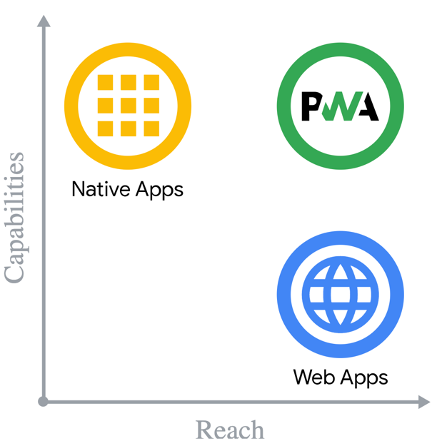
\includegraphics{./img/WatIsEenPwa.png}
	\caption{voorstelling wat een PWA is \autocite{Richard2020}}
	\label{fig:watIsEenPWA}
\end{figure}


\subsection{Service workers}

	De service worker is een script dat veel functionaliteiten beschikbaar maakt die voordien enkel beschikbaar waren voor native applicaties. In dit hoofdstuk wordt er bekeken welke functionaliteiten de service worker juist beschikbaar maakt voor een PWA en hoe dit gebeurt. 
	
	
	
	\subsubsection{Wat is een service worker}
	\label{ch: Wat is een servcie worker}
	
		Een service worker is een web worker die tussen het netwerk en de applicatie wordt geplaatst. Dit zorgt ervoor dat de service worker inkomende en uitgaande netwerkverzoeken kan controleren en eventueel manipuleren.
		\autocite{Mozilla2020}
		
		Een web worker is een script dat in de achtergrond van een applicatie werkt en die onafhankelijk is van de andere scripts. Web workers hebben dus geen impact op de prestaties van de webapplicatie die er gebruik van maakt.  Web workers hebben geen toegang tot het Document Object Model (DOM) van een webapplicatie, ze kunnen de inhoud van een website dus niet rechtstreeks manipuleren.
		\autocite{Verdu2015}
		\autocite{Hiltunen2018}
		
		
		Services workers werken dus constant op de achtergrond, maar de manier waarop service workers opgebouwd zijn (
		zie hoofdstuk \ref{ch: Wat is een servcie worker}) heeft geen significante invloed op de batterijduur van een mobiel toestel.
		\autocite{Malavolta2016}
	
	
	\subsubsection{Functionaliteiten die een service worker mogelijk maakt}
	\label{ch: Functionaliteiten die een serivce worker mogelijk maakt}
	
		De service worker werkt onafhankelijk van de applicatie. Dit houdt in dat een service worker wel nog kan werken terwijl de applicatie afgesloten is. Hierdoor zijn volgende functies mogelijk binnen een webapplicatie:
	
		
		
		\subparagraph{Offline gebruik}
		
			Als een PWA voor een eerste keer geladen wordt op een toestel zullen de bezochte pagina's offline beschikbaar blijven. Dit gebeurt door de  HTML, CSS en JavaScript bestanden die nodig zijn om de pagina's te creëren lokaal op te slaan. Applicaties die geen gebruik maken van netwerkverzoeken om data te laden, zullen dus offline volledig werken.
			
			Met service workers kunnen netwerkverzoeken en pagina's ook gecached worden. Als een pagina geladen wordt, kunnen alle elementen opgeslagen worden op het toestel. Als deze pagina later opnieuw bezocht wordt, hoeft deze niet meer aan de server gevraagd te worden. Hierdoor wordt de applicatie sneller en minder afhankelijk van de netwerkverbinding.
			Volgens onderzoek, dat uitgevoerd werd door Google, verlaten 53\% procent van de gebruikers een website als deze niet geladen is binnen 3 seconden. Service workers kunnen dus helpen om het aantal gebruikers op jouw website te verhogen.
			\autocite{Google2017}
			
			De twee mechanismes die gebruikt worden om data offline beschikbaar te maken zijn ‘indexedDB’ en de ‘cache API’.
			\autocite{Osmani2019}
			\autocite{Mozilla2020a}
			
			Cache API: \\

				De cache API wordt gebruikt om data die verkregen werd van netwerkverzoeken op te slaan. Zowel de ‘request’ als de ‘response’ van een netwerkverzoek kunnen in de cache API opgeslagen worden.
				\autocite{Scales2019}

			IndexedDB: \\

				IndexedDB is een mechanisme dat gebruikt wordt om lokaal gestructureerde data op te slaan. Het kan vergeleken worden met object georiënteerde databasemanagementsystemen die gebruik maken van JavaScript objecten om data op te slaan. Een IndexedDB maakt gebruik van indexen. Dit heeft als voordeel dat het uitlezen van data snel kan gebeuren.
				\autocite{Mozilla2019}
	
	
	\subparagraph{Notificaties}
	
		Er zijn twee soorten notificaties: lokale notificaties en push notificaties. 
		
		Lokale notificaties worden geactiveerd vanop de applicatie van de gebruiker, er zijn geen externe invloeden die deze notificatie activeren.
		
		Binnen lokale notificaties kunnen we nog het onderscheid maken tussen persistente en niet-persistente notificaties.
		Niet-persistente notificaties zijn notificaties die enkel getoond kunnen worden als de applicatie geopend is. Dit type notificaties heeft geen service worker nodig. 
		Persistente notificaties zijn notificaties die nog steeds geactiveerd worden vanuit de code op het toestel, maar de applicatie moet niet meer actief zijn. Hier is wel een service worker nodig.
	
		Push notificaties worden niet geactiveerd binnen de applicatie, maar worden geactiveerd door een server.
		Om push notificaties te gebruiken, moet er gebruik gemaakt worden van twee web-API's: de notifications API en de push API.
		
		Notifications API: \\
		
			Dit is een API die het uiterlijk en het gedrag van een notificatie zal bepalen. Deze API wordt zowel gebruikt voor lokale als voor push notificaties.
			Om gebruik te maken van deze API moet de gebruiker expliciet toegang geven aan de applicatie.
			
			Een voorbeeld van de code van een notificatie kan er als volgt uitzien: 
		
\begin{lstlisting}
function displayNotification() {
  if (Notification.permission == 'granted') {
   navigator.serviceWorker.getRegistration().then(function(reg) {
     var options = {
       body: 'Here is a notification body!',
       icon: 'images/example.png',
       vibrate: [100, 50, 100],
       data: {
         userId: “383209489398274”
       },
       actions: [
         {action: 'explore', title: 'Explore this new world',
           icon: 'images/checkmark.png'},
         {action: 'close', title: 'Close notification',
           icon: 'images/xmark.png'},
       ]
     };
     reg.showNotification('Hello world!', options);
   });
  }
}
\end{lstlisting}
			Om een notificatie weer te geven, wordt er een object verwacht waar de inhoud van de melding wordt vastgelegd. De mogelijke eigenschappen die aan het object kunnen meegeven worden staan beschreven in tabel \ref{tabelNotification}
			
			\begin{table}[H]
				\centering
				\begin{tabular}{cp{12cm}}
			       body & De boodschap die in de melding staat.  \\
			       icon & Het icoontje dat in de notificatie wordt getoond. \\
			       vibrate & Het vibratiepatroon dat de melding zal maken in milliseconden. \\
			       data & Data is een object dat gebruikt kan worden als de gebruiker op de notificatie  klikt. Dit object zal dan ontvangen worden in de applicatie. Hier zal vaak het id van de gebruiker teruggevonden worden. \\
			       actions & Er kunnen ook acties toegevoegd worden aan de melding. Elk object in deze array zal een knop worden op de melding met een andere functie. Het gedrag van de knoppen wordt bepaald in de applicatie aan de hand van de ‘action’. \\
				\end{tabular}	
				\caption{beschrijving Notifications API}
				\label{tabelNotification}
			\end{table}
			\autocite{Developers2019}
			\autocite{Mozilla2019a}
			

			Push API:	\\
	
				
			De push API wordt gebruikt door de service worker. Als de server een notificatie verstuurt, wordt deze opgevangen door de push API. Deze API zal dan gebruik maken van de notifications API om een melding op het toestel van de eindgebruiker te tonen.
			\autocite{Mozilla2019b}
			\autocite{Gaunt2020}
	
		\subparagraph{Achtergrondsynchronisatie }
		Een PWA kan gebruik maken van de background sync API om achtergrondsynchronisatie toe te passen.
		
		Achtergrondsynchronisatie kan toegepast worden als er een trage of geen netwerkverbinding is. 
		
		Achtergrondsynchronisatie is het proces waarbij een netwerkverzoek, dat uitgevoerd werd als er geen of een te zwakke internetverbinding was, wordt opgeslagen in de service worker en wordt uitgevoerd als er wel een stabiele internetconnectie is.
	
		Een toepassing die hier gebruik kan van maken zijn sociale media platformen. Als het bericht verzonden wordt terwijl de gebruiker offline is, zal er geen fout getoond worden maar zal dit bericht verzonden worden vanaf er internet is.
		
		Google Chrome op Android maakt hier gebruik van. Als er een website bezocht wordt als er geen internetverbinding is, krijgt de gebruiker de melding: "Chrome laat je weten wanneer de pagina klaar is" (zie figuur \ref{fig:backSync1}). Vanaf dat het toestel terug een internetverbinding heeft, en het de pagina heeft kunnen downloaden, zal de gebruiker een melding krijgen met de boodschap dat de pagina bekeken kan worden (zie figuur \ref{fig:backSync2}).
	
	
		\begin{figure}[H]
			\centering
			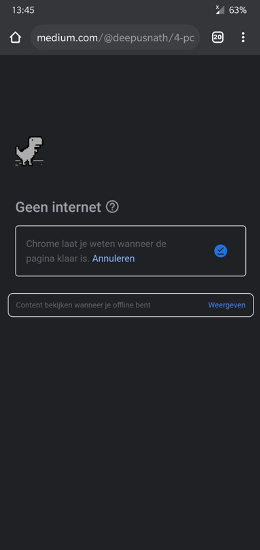
\includegraphics[width=35mm]{./img/backSync1.png}{}
			\caption{achtergrond synchronisatie bij Google Chrome op Android - pagina offline}
			\label{fig:backSync1}
		\end{figure}
		
		\begin{figure}[H]
			\centering
			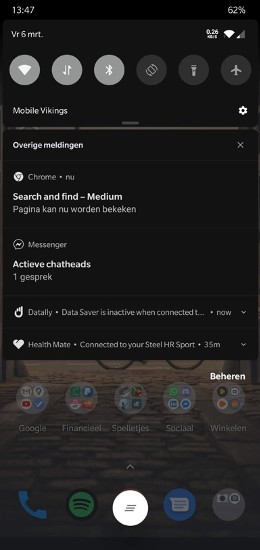
\includegraphics[width=35mm]{./img/backSync2.png}
			\caption{achtergrond synchronisatie bij Google Chrome op Android - melding als gebruiker terug online is}
			\label{fig:backSync2}
		\end{figure}
		\subsubsection{Service worker lifecycle }
			De levenscyclus van de service worker is onafhankelijk van de levenscyclus van de webapplicatie. Als de webapplicatie gesloten wordt, blijft de service worker gewoon werken.
			
			Om een service worker te installeren, moet deze geregistreerd worden in de JavaScript van de webapplicatie. Dit gebeurt normaal bij het eerste bezoek aan de website van de gebruiker.
			
\begin{lstlisting}
function displayNotification() {
if ('serviceWorker' in navigator) {
	navigator.serviceWorker.register('/service-worker.js');
}
\end{lstlisting}
	
		Als een service worker wordt geïnstalleerd, worden de opgegeven statische bestanden (foto’s, css-bestanden, JavaScript-bestanden) gedownload. Als dit slaagt, wordt er naar de activatiefase gegaan, als dit niet slaagt zal dit proces zich herhalen tot het slaagt. 
		
		Tijdens de activatiefase wordt er bekeken welke gecachete gegevens geüpdatet moeten worden en welke niet. De service worker zal de bestanden die het ontvangen heeft van het eerste netwerkverzoek vergelijken met zijn huidig cachegeheugen. Als er verschillen zijn, zal dit cachegeheugen aangepast worden.
		
		Als de activatiefase geslaagd is, heeft de service worker controle over de pagina's die binnen zijn scope vallen. Deze scope moet gedefinieerd worden binnen de service worker.
		
		Nu het oude cachegeheugen up-to-date is, zal de service worker overgaan naar een “rust”-toestand, hierbij wacht de service worker op netwerkverzoeken van bestanden die binnen zijn scope vallen.
		
		Als er een netwerkverzoek wordt verstuurd, zal de service worker deze verzoeken afhandelen. Na een bepaalde tijd zal de service worker terug naar de ‘rust’-modus gaan tot er een nieuw netwerkverzoek is. De service worker gaat naar deze ‘rust’-toestand om zowel cpu-kracht als geheugen te sparen.
		\autocite{Gaunt2019}
		
		Dit proces wordt geïllustreerd in van figuur \ref{fig:swLifeCycle}
		
		
		\begin{figure}[H]
			\centering
			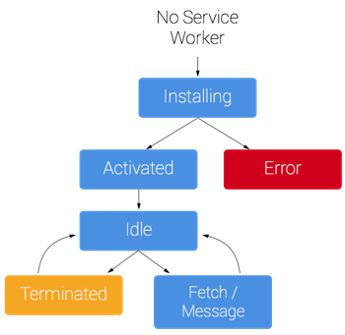
\includegraphics{./img/ServiceWorkerLifeCycle.png}
			\caption{schema levenscyclus van een service worker \autocite{Gaunt2019}}
			\label{fig:swLifeCycle}
		\end{figure}
	

\subsection{A2HS}

	
	Als een applicatie voldoet aan bepaalde criteria, kan deze geïnstalleerd worden op het toestel van de gebruiker. Deze functie is beschikbaar voor verschillende besturingssystemen: Windows, macOS, Android, iOS.
	
	Een website moet voldoen aan volgende criteria:
	
	\begin{itemize}
		\item	Nog niet geïnstalleerd zijn
		\item	Een HTTPS-connectie hebben
		\item	Een manifest.json bestand hebben
		\item	Een service worker registreren.
	\end{itemize}
	
	Als een website aan alle criteria voldoet zal er een beforeinstallprompt event gestart worden. Elke browser gaat hier anders mee om. 
	Zo is in figuur \ref{fig:A2HSWindows} te zien dat er een icoontje komt in de adresbalk in Google Chrome voor computers. Bij Google Chrome op mobiele toestellen zal er onderaan het scherm een banner komen (zie figuur \ref{fig:A2HSAndroid}).
	
	\begin{figure}[H]
		\centering
		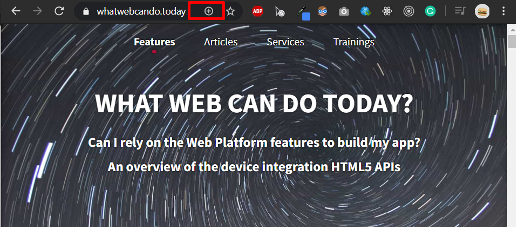
\includegraphics{./img/beforeinstallprompt_windows.png}	
		\caption{beforeinstallprompt in Google Chrome op Windows 10}
		\label{fig:A2HSWindows}
	\end{figure}
	
	\begin{figure}[H]
		\centering
		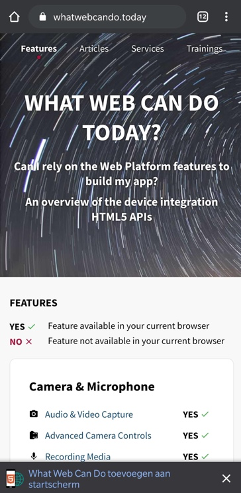
\includegraphics{./img/beforeinstallprompt_android.png}
		\caption{beforeinstallprompt in Google Chrome op Android}
		\label{fig:A2HSAndroid}
	\end{figure}
	
	Op Apple toestellen (iPhone, Mac) heeft het beforeinstallprompt geen effect. De gebruiker moet zelf op zoek gaan in het menu om de applicatie te installeren.
	Niet alle gebruikers zullen weten hoe ze dit moeten doen, het is dus aangeraden om de gebruiker hierin te begeleiden door hem duidelijke instructies te geven.
	\autocite{PWAbuilder2020}


\subsection{Application shell}
	De application shell of app shell is de minimale HTML, CSS en JavaScript die nodig is om een userinterface te tonen op een toestel. Dit is vaak de header, footer en de navigatie.
	
	Figuur \ref{fig:AppShell} maakt het verschil duidelijk tussen de application shell en de content.
	
	Door de bestanden die steeds terugkomen offline op te slaan, worden deze veelgebruikte elementen onmiddellijk geladen. Dit zorgt ervoor dat een webapplicatie meer zal aanvoelen als een native applicatie.
	
	Het toepassen van deze architectuur biedt een aantal voordelen:
	
	\begin{itemize}
		\item	Consistent snel
		\item	Voelt native aan
		\item	De gebruiker moet minder data downloaden
	\end{itemize}
	\autocite{Osmani2019a}
	
	\begin{figure}[!htb]
		\centering
		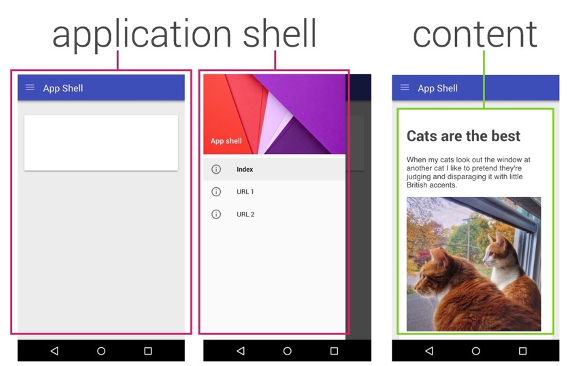
\includegraphics{./img/ApplicationShell.png}
		\caption{application shell architectuur \autocite{Osmani2015}}
		\label{fig:AppShell}
	\end{figure}
	
\newpage
\subsection{Progressive enhancement}
	Progressive enhancement is een strategie bij webontwikkeling waarbij er gezorgd wordt dat alle hoofdfunctionaliteiten beschikbaar zijn op alle toestellen. Meer geavanceerde functies worden aan deze basisversie toegevoegd. 
	
	Het doel van progressive enhancement is dat een applicatie gebruikt kan worden op elk toestel en dat meer modernere toestellen of browsers van een rijkere ervaring kunnen genieten.
	\autocite{Vanhala2017}
	
	
\subsection{Application manifest}
	Het web app manifest is een JSON-bestand dat informatie bevat over de applicatie. Deze informatie is nodig voor het installeren van een PWA op een toestel.
	Aan de hand van dit bestand weet het besturingssysteem bijvoorbeeld welk icoon er gebruikt moet worden en hoe het startscherm er moet uitzien.
	
	Voorbeeld van een minimum app manifest voor de Google Maps PWA.
	
\begin{lstlisting}
{
	"short_name": "Maps",
	"name": "Google Maps",
	"icons": [
		{
			"src": "/images/icons-192.png",
			"type": "image/png",
			"sizes": "192x192"
		},
		{
			"src": "/images/icons-512.png",
			"type": "image/png",
			"sizes": "512x512"
		}
	],
	"start_url": "/maps/?source=pwa",
	"background_color": "#3367D6",
	"display": "standalone",
	"scope": "/maps/",
	"theme_color": "#3367D6"
}
\end{lstlisting}
	
	\newpage
		Tabel \ref{tabelManifest} beschrijft de attributen van een minimum app manifest.
	
		\begin{table}[H]
			\centering
			\begin{tabular}{cp{12cm}}
	     		short\_name & Naam van de applicatie die op het startscherm gebruikt zal worden. Deze mag maximaal 12 karakters lang zijn. \\
	     		name & Naam die op alle andere plekken gebruikt zal worden: vb. bij de vraag of de app geïnstalleerd mag worden. Deze mag maximaal 45 karakters lang zijn. \\
	     		icons & Een lijst vna objecten die het icoon bepaalt dat de applicatie zal gebruiken. Verschillende platformen vragen verschillende types iconen Dit object heeft volgende eigenschappen:
		     		\begin{itemize}
			    		  \item src - bron van het icoon
			    		  \item type - het bestandstype van het icoon
			    		  \item size - de afmeting van het icoon
	     			\end{itemize} \\
	     		start\_url & De url naar waar de PWA moet gaan als de applicatie gestart wordt vanaf het startscherm van een toestel.\\
	     		background\_color & Hier wordt een kleur gedefinieerd. Dit kleur zal gebruikt worden voor het opstartscherm. \\
	     		display & Dit bepaalt in wat voor webview de PWA getoond zal worden. Mogelijkheden zijn:
		     		\begin{itemize}
			     		  \item fullscreen - opent de applicatie zonder UI-elementen (adresbalk, terug knop, ...)
			     		  \item standalone - opent de applicatie als een native applicatie los van de browser. Er worden geen UI-elementen van de browser getoond.
			     		  \item minimal-ui - opent de applicatie in de browser maar toont slechts beperkte UI elementen van de browser. De adresbalk is weg maar de ‘vorige’ knop is er nog.
			     		  \item browser - opent de PWA in een normaal browser tabblad.
		     		\end{itemize} \\
	     		scope & De scope bepaalt alle links die binnen de PWA vallen. \\
	     		theme\_color & De kleur die de adresbalk zal innemen.
			\end{tabular}	
			\caption{beschrijving minimum application manifest}
			\label{tabelManifest}
		\end{table}
				
			
	
	
	\autocite{LePage2020}

\subsection{Geschiedenis van PWA's}

	\subsubsection{"One last thing"}

		 “One last thing” is de zin waarmee Steve jobs, co-founder van Apple, zijn jaarlijkse toespraak steeds afsloot. Er volgde meestal een revolutionair idee of product dat Apple zal uitbrengen.
		
		In juni 2007 sloot Steve Jobs, nadat hij net de eerst iPhone had voorgesteld, zijn toespraak af met de visie die Apple toen had over hoe het web er moet uitzien. De term progressive web apps bestond nog niet, maar de concepten die hij uitlegde zijn wel de basis van PWA's. Steve Jobs citeerde volgende stellingen:
	
		
		\begin{itemize}
			\item \textit{ “We have got an inovative way to create applications for mobile devices, and it’s all based on the fact that iPhone has the full Safari engine on board”}
			\item \textit{“You can write apps that look like iPhone apps and that integrate with iPhone services”}
			\item \textit{“Instant distribution, just put them on the internet”}
			\item \textit{“They are really easy to update, just put the update on your server”}
		\end{itemize}
		\autocite{Jobs2007}
		
		Apple had verwacht dat dit een succes zou zijn. Maar de ontwikkelaars waren teleurgesteld, ze hadden verwacht dat ze meer toegang zouden krijgen tot de iPhone. In de eerste versie van de iPhone kon enkel gebruik gemaakt worden van de apps die geïnstalleerd waren door Apple, er konden geen nieuwe apps gedownload worden.
		\autocite{Strieb2016}
		
		 De visie van Apple veranderde echter toen ze het volgende jaar de app-store lanceerden. \autocite{Silver2018}
	 
	 \subsubsection{Crome dev summit 2015}
	 
		 Chrome dev summit is een conferentie voor webontwikkelaars georganiseerd door Google. 
		 
		 Alex Russel en Andreas Bovens gebruikten voor het eerst de term “Progressive Web Apps”. Op dit moment ondersteunde enkel Android service workers en A2HS.
		 
		 Ook werd het concept van de application shell voorgesteld.
		 \autocite{Russel2015}
	 
	 
	 \subsubsection{iOS 13}
		 Op 19 september 2019 stelde Apple iOS 13 voor. Deze software-update zorgde ervoor dat de iPhone gebruik kon maken van een service worker. De applicaties kunnen nu ook geïnstalleerd worden op het toestel, de gebruiker moet dit wel nog zelf doen aan de hand van het menu.
		 \autocite{Apple2020}
	 


\subsection{Voorbeelden van PWA's}
\label{ch: Voorbeelden}

	
	\subsubsection{Outlook}
		Google is niet de enige grote speler die PWA's wil promoten en implementeren.
		\autocite{Microsoft2020}
		
		Microsoft geeft het goede voorbeeld door de veelgebruikte e-mail-client Outlook ook beschikbaar te maken als een PWA.
		De PWA-versie van de applicatie is slechts 800KB groot (figuur \ref{outlookPWA}) terwijl de traditionele versie op een desktop 1,8GB groot is (figuur \ref{outlookMac}).
		\begin{figure}[H]
			\centering
			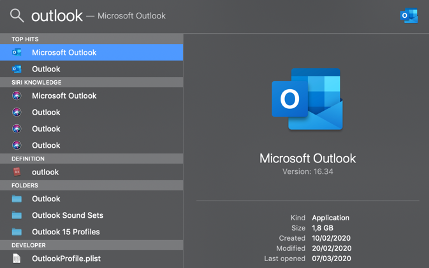
\includegraphics{./img/Outlook_native.png}
			\caption{Outlook op Mac}
			\label{outlookMac}
		\end{figure}
		
		\begin{figure}[H]
			\centering
			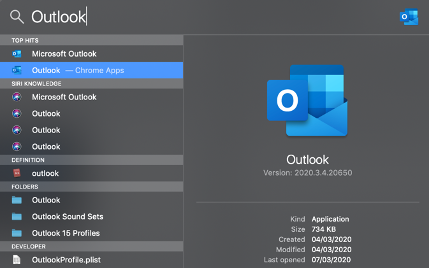
\includegraphics{./img/Outlook_pwa.png}
			\caption{Outlook op Mac als PWA}
			\label{outlookPWA}
		\end{figure}
		
	\subsubsection{AliExpress}
		
		AliExpress, één van de grootste e-commerce platformen, implementeerde hun website als een PWA. De resultaten waren heel positief, bij nieuwe gebruikers werd er 104\% meer verkocht. De gemiddelde gebruiker bleef ook 74\% langer op de website.
		\autocite{Developers2020}
	
	
	\subsubsection{Twitter}
	
		Twitter, één van de grootste sociale media platformen, implementeerde hun website ook als PWA. De resultaten waren ook hier positief. Het datagebruik van de gebruiker werd met 70\% verminderd. De gemiddelde gebruiker bekeek ook 65\% meer pagina's dan op de vorige website van Twitter.
		Het afdelingshoofd van ontwikkeling van Twitter deed volgende uitspraak over de PWA:
		
		\textit{Twitter Lite is now the fastest, least expensive, and most reliable way to use Twitter. The web app rivals the performance of our native apps but requires less than 3\% of the device storage space compared to Twitter for Android.}
		\autocite{Developers2020a}
		\autocite{Love2018}
	
	\subsubsection{Starbucks}
	
		Starbucks heeft een native applicatie waarmee er koffie of andere dranken besteld kunnen worden als ze in een Starbucks zaak zijn. Deze applicatie is populair bij klanten die vaak terugkomen naar Starbucks. Klanten die slechts eenmalig komen, willen vaak geen applicatie downloaden om deze maar éénmaal te gebruiken.
		
		Dit werd opgelost door de functionaliteit die de native applicatie biedt ook te implementeren als een PWA zodat deze gebruikt kan worden via het web zonder geïnstalleerd te worden.
		
		De klanten kunnen nu vanuit de website een bestelling personaliseren en bestellen. Hierdoor wordt er tijd gewonnen bij het bestellingproces.
		\autocite{Formidable2020}
		\autocite{Kawatka2020}
	
	\subsubsection{Uber}
	
		Uber is aan het uitbreiden naar nieuwe markten. Ze willen dat hun service ook beschikbaar wordt ongeacht de locatie, netwerkiOS of toestel van de gebruiker.
		
		Met deze drie parameters in gedachten hebben ze een alternatief gebouwd voor hun native mobiele applicatie. Deze website kan bezocht worden op m.uber.com.
		
		Het grootste doel was om de website snel te laten werken op ‘low-end’ toestellen met een 2g connectie. 
		\autocite{Croll2017}
	
	\subsubsection{Pinterest}
	
		Pinterest zag aan de hand van hun analytics dat slechts 1\% van de niet geregistreerde bezoekers op hun vorige site een account aanmaakte. Dit probleem hebben ze opgelost aan de hand van een PWA.
		Na het implementeren van de PWA steeg het aantal registraties met 60\% en het aantal sessies van langer dan 5 minuten steeg met 40\%.
		\autocite{Osmani2019b}
		
		
	\subsubsection{The coronavirus app}
	
		Deze thesis is geschreven op het moment van de corona-crisis. The coronavirus app is een PWA waar real-time data in verband met het virus kan geraadpleegd worden. 
		Deze PWA was tijdens de eerste dagen van de uitbraak al online. Dit bewijst hoe snel een PWA online gepubliceerd kan worden.
		Na de eerste release van de applicatie werden er dagelijks nieuwe functionaliteiten toegevoegd. 
		Deze PWA was een van de eerste informatiebronnen die voor iedereen beschikbaar was. De applicatie had meer dan 10 miljoen actieve gebruikers. 
		
		
\clearpage
\section{Besturingssystemen en PWA's}
	\label{ch: BesturingssystemenEnPWAs}
	
	Om te weten te komen voor welke toepassingen een PWA gemaakt kan worden en voor welke toepassingen nog steeds een native applicatie nodig is, is het belangrijk om te weten wat de technische mogelijkheden zijn van een PWA. In deze sectie van de literatuurstudie wordt er bekeken welke functies, die beschikbaar zijn voor native applicaties, al dan niet gebruikt kunnen worden door PWA's.
	
	Aan het einde van dit hoofdstuk zal er een overzicht gevormd worden met alle functionaliteiten die een PWA kan implementeren (\ref{concTabel}).
	
	Dit onderzoek werd gevoerd met behulp van de website \href{https://whatwebcando.today/}{whatwebcando.today} en
	\href{https://caniuse.com/}{caniuse.com}.
	
	                                 
	\href{https://whatwebcando.today/}{whatwebcando.today} is een website die kleine voorbeelden van verschillende technologieën demonstreert. Door deze voorbeelden te testen op verschillende platformen kan er uitgemaakt worden welke technologieën er beschikbaar zijn voor het web, en op welke platformen deze beschikbaar zijn.
	
	\href{https://caniuse.com/}{ caniuse.com} is een website die voor verschillende web-technologieën een overzicht biedt op welke browsers deze technologie gebruikt kan worden en op welke niet. Deze website werd gebruikt om de ondervindingen van de testen die werden uitgevoerd te valideren. 
	
	Een web-API is een API die wordt aangeboden door de browser. Het verschil met web-API's en traditionele API's is dat web-API's lokaal worden aangeboden door de browser en er dus geen internetverbinding nodig is om van deze functionaliteiten te genieten.
	\autocite{Mozilla2019c}
	
	
	Als er meer informatie nodig was over de web API's werd deze gevonden op \href{https://developers.google.com/}{developers.google.com } of op \href{https://developer.mozilla.org/nl/}{MDN web docs}.
	
	Er werd gekeken op welke platformen bepaalde functies wel en niet werkten. Volgende platformen werden onderzocht:
	\begin{itemize}
	   \item Desktop:
	   \begin{itemize}
	     \item	Microsoft Edge versie 80 op Windows 10
	     \item	Mozilla Firefox versie 73.0 op Windows 10
	     \item	Google Chrome versie 79.0 op Windows 10
	     \item  Safari (desktop) versie 13.0.5 op een Macbook Pro met macOS Mojave (10.14.6)
	   \end{itemize}
	\end{itemize}
	
	
	\begin{itemize}
	   \item Mobiel:
	   \begin{itemize}
	     \item Google Chrome versie 80 op Android 10 op een OnePlus 6
	     \item Safari (mobiel) versie 13 op iOS 13 op een iPhone SE 
	     
	   \end{itemize}
	\end{itemize}
	
	De testen werden uitgevoerd op 7 maart 2020.
	
	De website \href{https://whatwebcando.today/}{whatwebcando.today} geeft een overzicht van de functionaliteiten aan de hand van een bepaalde structuur. Deze structuur werd overgenomen en ziet er als volgt uit:
	   \begin{itemize}
	     \item	Media
	     \item	Verbinding
	     \item	Toestel kenmerken
	     \item	Native gedrag
	     \item	Besturingssysteem
	     \item	Input
	     \item	User experience
	     \item	Locatie en positionering
	     \item	Scherm en output
	   \end{itemize}
	
	\subsection{Onderzoek}
	
	\subsubsection{Media}
	
	\paragraph{Video met audio }
	
	Sommige van de meest populaire mobiele applicaties zijn sterk afhankelijk van camera-functionaliteit. Voorbeelden hiervan zijn Snapchat, Instagram, Messenger, WhatsApp, ...
	
	Bij deze applicaties is het belangrijk dat de camera aan volgende vereisten voldoet:
	
	   \begin{itemize}
	     \item	Snel en eenvoudig te gebruiken
	     \item	Er moet van camera gewisseld kunnen worden
	     \item	Er moet ingezoomd kunnen worden
	     \item	De flashlight moet gebruikt kunnen worden
	   \end{itemize}
	
	De media capture API \autocite{DzungDTran2012}  maakt het mogelijk om een video die opgenomen wordt met de camera van het toestel te tonen op de webpagina. Deze video kan dan opgeslagen worden in de code en verzonden worden naar een server. 
	\autocite{Fransson2017}
	
	De media capture API is ook in staat om aan het toestel te vragen welke camera's er beschikbaar zijn en dan te verwisselen van camera.
	\autocite{Scales2020a}
	
	Ook meer geavanceerde functionaliteiten  zijn beschikbaar. Het gedrag van de zoom en de flashlight kan ook programmatisch bepaald worden.
	\autocite{Oberhofer2017} \autocite{Ogundipe2018}
	
	
	Al de belangrijkste functionaliteiten die een gebruiker verwacht, zijn allemaal aanwezig. Applicaties die afhankelijk zijn van video-opnames kunnen dus geïmplementeerd worden als PWA.
	
	\begin{table}[H]
		\centering
		\begin{tabular}{llllll}
			Edge & Firefox & Chrome & Safari & Android (Chrome) & iOS (Safari) \\
			Ja   & Ja      & Ja     & Ja     & Ja               & Ja          
		\end{tabular}	
		\caption{ondersteuning van de Media Capture API op 7 maart 2020}
	\end{table}
	
	
	
	\paragraph{Foto's }
	
	Het vastleggen van foto's is ook voor veel populaire applicaties belangrijk. Ook dit is een belangrijke functionaliteit voor sociale media applicaties.
	
	Foto's die gedeeld worden op sociale media moeten vaak van een zo hoog mogelijke kwaliteit zijn. Op native applicaties wordt deze kwaliteit bereikt door volgende eigenschappen: 
	
	 \begin{itemize}
	     \item Manuele en automatische focus
	     \item Aanpassen van sluiteriOS
	     \item Aanpassen van witbalans
	     \item Aanpassen ISO-waarde
	     \item Gebruik maken van HDR 
	   \end{itemize}
	
	Foto's kunnen ook, net zoals een video, genomen worden aan de hand van de Media Capture API. Deze API is echter niet in staat om deze instellingen van de camera aan te passen.
	
	De Image Capture API \autocite{Mandyam2017} is ontwikkeld om meer controle te hebben over de camera. Deze API zorgt ervoor dat instellingen zoals witbalans, temperatuur, exposure, ISO, helderheid, contrast, saturatie en zoom programmatisch aangepast kunnen worden.
	
	Deze API heeft standaard geen ondersteuning voor HDR, maar dit kan zelf geïmplementeerd worden aan de hand van ‘third-party-packages’.
	\autocite{Bhaumik2019}
	
	\begin{table}[H]
		\centering
		\begin{tabular}{llllll}
			Edge & Firefox & Chrome & Safari & Android (Chrome) & iOS (Safari) \\
			Nee   & Nee      & Ja     & Nee     & Ja               & Nee          
		\end{tabular}	
		\caption{ondersteuning van de Image Capture API op 7 maart 2020}
	\end{table}
	
	
	
	\paragraph{Geluidopname }
	De Mediarecorder API, \autocite{CasasSanchez2017} door meerdere browsers aangeboden, is een manier om eenvoudig geluidsfragmenten op te nemen en te importeren in een webapplicatie.
	
	Helaas is er voor Apple-toestellen geen ondersteuning. In de toekomst zal deze functie waarschijnlijk ook beschikbaar worden voor deze toestellen. Dit wordt in de volgende versie van Safari (Safari 14) voor desktop en iOS verwacht. Voor Safari voor iOS bestaat deze functie al maar is het nog een experimentele functie die de gebruiker zelf moet activeren.
	
	
	
	\begin{table}[H]
		\centering
		\begin{tabular}{llllll}
			Edge & Firefox & Chrome & Safari & Android (Chrome) & iOS (Safari) \\
			Ja   & Ja      & Ja     & Nee     & Ja               & Nee          
		\end{tabular}	
		\caption{ondersteuning van de Mediarecorder API op 7 maart 2020}
	\end{table}
	
	Gelukkig is er een alternatief voorzien met HTML5-tags. Dit is een methode die voor alle platformen zal werken maar niet op dezelfde manier.
	
	\begin{lstlisting}
	<input type="file" accept="audio/*" capture>
	\end{lstlisting}
	
	Er wordt gebruik gemaakt van een inputveld waar de gebruiker een bestand kan uploaden. Door het accept attribuut wordt duidelijk gemaakt dat enkel audiofragmenten geüpload mogen worden. Het capture attribuut zorgt ervoor dat waar mogelijk de gebruiker een audiofragment kan opnemen in de default geluidsopname app. Dit fragment wordt dan automatisch geïmporteerd in de webapplicatie. Dit is enkel mogelijk op mobiele toestellen en dus niet in desktopbrowsers.
	\autocite{Kinlan2019}
	
	Dit is een goed voorbeeld van progressive enhancement. 
	
	
	
	\paragraph{Real-time communicatie }
	
	Bij de meeste populaire communicatieapplicaties zoals WhatsApp, Messenger, Skype, ... is videobellen mogelijk. Om dit mogelijk te maken, moet er live video en audio gestreamd kunnen worden tussen twee of meer personen.
	
	‘Real-time communication in the web’ of WebRTC \autocite{Jennings2019} is een verzameling van API's die het verzenden en ontvangen van real-time video en audio mogelijk maakt, zonder afhankelijk te zijn van een gecentraliseerde server. Deze server is echter wel nodig om een connectie tot stand te brengen. Eens deze connectie er is, is er een peer-to-peer verbinding.
	
	\begin{table}[H]
		\centering
		\begin{tabular}{llllll}
			Edge & Firefox & Chrome & Safari & Android (Chrome) & iOS (Safari) \\
			Ja   & Ja      & Ja     & Ja     & Ja               & Ja          
		\end{tabular}	
		\caption{ondersteuning van WebRTC op 7 maart 2020}
	\end{table}
	
	
	
	
	\paragraph{Casting}
	
	Applicaties die media tonen aan de gebruiker kunnen deze casten naar een tv-toestel. Dit gebeurt bij Apple-toestellen aan de hand van Airplay en bij Android-toestellen aan de hand van Google cast.
	
	YouTube is een applicatie die hier gebruik van maakt. Als er een video bekeken wordt, zal de gebruiker een optie krijgen om deze te tonen op een tv.
	
	Op Apple-toestellen kan een PWA nu ook AirPlay implementeren. 
	\autocite{Apple2020a}
	
	De Chrome Sender API \autocite{Developers2020b} zorgt ervoor dat toestellen media kunnen delen op een tv of ander scherm die dit ondersteunt.
	
	\begin{table}[H]
		\centering
		\begin{tabular}{llllll}
			Edge & Firefox & Chrome & Safari & Android (Chrome) & iOS (Safari) \\
			Nee   & Nee      & Nee     & Ja     & Nee               & Ja          
		\end{tabular}	
		\caption{ondersteuning Apple AirPlay op 7 maart 2020}
	\end{table}
	\begin{table}[H]
		\centering
		\begin{tabular}{llllll}
			Edge & Firefox & Chrome & Safari & Android (Chrome) & iOS (Safari) \\
			Ja   & Ja      & Ja     & Ja     & Ja               & Ja          
		\end{tabular}	
		\caption{ondersteuning van Chrome Sender API op 7 maart 2020}
	\end{table}
	
	
	
	
	\paragraph{Media-controle in de notificatie }
	
	
	Als een native applicatie media afspeelt op een mobiel toestel, kan deze applicatie bestuurd worden vanuit de notificatie. De afgespeelde media zal ook niet stoppen als een gebruiker de applicatie verlaat.
	
	Een voorbeeld hiervan is Spotify. In de notificatie van Spotify kan de gebruiker volgende acties uitvoeren.
	 \begin{itemize}
	   \item	Informatie bekijken over het nummer
	   \item	Naar het volgende nummer gaan
	   \item	Het nummer pauzeren
	   \item	Het nummer toevoegen aan “mijn favorieten”
	   \item	De vooruitgang van het nummer zien en aanpassen
	\end{itemize}
	De Media Session API \autocite{Beaufort2019} zorgt ervoor dat als er media afgespeeld wordt op een website, en de browser wordt gesloten, de media niet zal stoppen met afspelen.
	
	Deze API zorgt er ook voor dat er een notificatie komt waar de gebruiker controle heeft over de afgespeelde media. 
	
	%Het voorbeeld van Spotify kan dus geïmplementeerd worden als PWA.
	
	\begin{table}[H]
		\centering
		\begin{tabular}{llllll}
			Edge & Firefox & Chrome & Safari & Android (Chrome) & iOS (Safari) \\
			Ja   & Ja      & Ja     & Ja     & Ja               & Ja          
		\end{tabular}	
		\caption{ondersteuning van Media Session API op 7 maart 2020}
	\end{table}
	
	
	
	\subsubsection{Connectie met andere apparaten}
	
	
	
	\paragraph{Bluetooth }
	
	Native applicaties kunnen een verbinding maken met bluetooth-toestellen. Eens er een verbinding is, kan er informatie uitgewisseld worden tussen de toestellen. Een voorbeeld van een applicatie die hier gebruik van maakt is de ‘Sony Headphones’ app. Aan de hand van deze app kan er verbinding gemaakt worden met een koptelefoon en kunnen de instellingen van de koptelefoon aangepast worden.
	
	Met de Web Bluetooth API \autocite{Grant2020} kan er vanuit de browser verbinding gemaakt worden met bluetooth-toestellen. De web API heeft zowel schrijf- als leesrechten bij externe toestellen. 
	
	Er kan dus geconcludeerd worden dat de Web Bluetooth API kan gebruikt worden voor applicaties die gebruik moeten maken van bluetooth-toestellen.
	\autocite{Beaufort2019a}
	
	\begin{table}[H]
		\centering
		\begin{tabular}{llllll}
			Edge & Firefox & Chrome & Safari & Android (Chrome) & iOS (Safari) \\
			Ja   & Nee      & Ja     & Nee     & Ja               & Nee          
		\end{tabular}	
		\caption{ondersteuning van Web Bluetooth API op 7 maart 2020}
	\end{table}
	
	
	
	\paragraph{USB}
	
	Verkopers van toestellen met USB kunnen nu gebruik maken van de Web USB API, \autocite{Rockot2020}. Bij het verbinden van een USB-toestel kan er automatisch een website geopend worden waarmee het toestel kan interageren.
	 
	Dit kan interessant zijn voor toestellen die een eenmalige set-up nodig hebben. Met deze technologie kan vermeden worden dat er overbodige software moet geïnstalleerd worden op het toestel van de gebruiker. 
	
	Dit is echter enkel mogelijk met een beperkt aantal browsers en er moet een HTTPS-verbinding zijn.
	\autocite{Beaufort2019b}
	
	\begin{table}[H]
		\centering
		\begin{tabular}{llllll}
			Edge & Firefox & Chrome & Safari & Android (Chrome) & iOS (Safari) \\
			Ja   & Nee      & Ja     & Nee     & Ja               & Nee          
		\end{tabular}	
		\caption{ondersteuning van Web USB API op 7 maart 2020}
	\end{table}
	
	
	\paragraph{NFC}
	
	Near Field Communication of NFC is een technologie om een kleine hoeveelheid informatie uit te wisselen over een kleine afstand (Maximum 20cm). NFC wordt gebruikt om draadloze betalingen uit te voeren met een betaalkaart of met een smartphone. 
	\autocite{Paus2007}
	
	\begin{table}[H]
		\centering
		\begin{tabular}{llllll}
			Edge & Firefox & Chrome & Safari & Android (Chrome) & iOS (Safari) \\
			Nee   & Nee      &  Nee     & Nee     & Nee               & Nee          
		\end{tabular}	
		\caption{ondersteuning van Web NFC API op 7 maart 2020}
	\end{table}
	
	Dit is een functie met veel mogelijkheden die helaas niet beschikbaar is voor webapplicaties.
	Er bestaat echter wel een API om gebruik te kunnen maken van NFC \autocite{RohdeChristiansen2020}, maar de Web NFC API is een experimentele API. Dit betekent dat de eindgebruiker dit nog niet kan gebruiken.
	
	
	
	\subsubsection{Toestelkenmerken}
	
	
	\paragraph{Netwerkinformatie}
	
	De Network information API \autocite{Lamouri2014} voorziet informatie over het type netwerkverbinding die de gebruiker momenteel bezit. Deze informatie bevat het connectietype (2g, 3g, 4g) en de maximale downloadiOS van deze verbinding.
	
	\begin{table}[H]
		\centering
		\begin{tabular}{llllll}
			Edge & Firefox & Chrome & Safari & Android (Chrome) & iOS (Safari) \\
			Nee   & Nee      &  Ja     & Nee     & Ja               & Nee          
		\end{tabular}	
		\caption{ondersteuning van Network Information API op 7 maart 2020}
	\end{table}
	
	\paragraph{Online status}
	
	Dit is een eenvoudige eigenschap die kan opgeroepen worden op het navigator object. Deze eigenschap bevat een booleaanse waarde die “waar” zal zijn als de gebruiker een connectie heeft met het internet. 
	
	Dit is een belangrijke eigenschap bij applicaties die real-time data gebruiken. Als de internetconnectie van de gebuiker wegvalt, kan er een melding  getoond worden. Op deze manier weet de gebruiker dat de data mogelijks niet up-to-date is.
	\begin{table}[H]
		\centering
		\begin{tabular}{llllll}
			Edge & Firefox & Chrome & Safari & Android (Chrome) & iOS (Safari) \\
			Ja   & Ja      &  Ja     & Ja     & Ja               & Ja          
		\end{tabular}	
		\caption{ondersteuning online status op 7 maart 2020}
	\end{table}
	
	\paragraph{Vibratiemotor }
	
	De Vibration API \autocite{Kostionen2018} zorgt ervoor dat de vibratiemotor kan aangesproken worden vanuit de webapplicatie.
	
	\begin{table}[H]
		\begin{tabular}{llllll}
			Edge & Firefox & Chrome & Safari & Android (Chrome) & iOS (Safari) \\
			Ja   & Ja      &  Ja     & Nee     & Ja               & Nee          
		\end{tabular}	
		\caption{ondersteuning vibratiemotor  op 7 maart 2020}
	\end{table}
	
	
	\paragraph{Batterijstatus}
	
	Aan de hand van de Battery Status API \autocite{Kostiainen2016} kan er informatie over de batterij van het toestel verkregen worden.
	
	Volgende informatie kan verkregen worden:
	 \begin{itemize}
		\item	Aan het opladen
		\item	Batterijpercentage
		\item	Bij opladen, tijd tot volladen
		\item	Bij niet opladen, tijd tot batterij leeg
	\end{itemize}
	
	Aan de hand van deze API kunnen er ook acties uitgevoerd worden op basis van het veranderen van de toestand van de batterij. Er kan bijvoorbeeld een functie uitgevoerd worden als de gebruiker zijn toestel met een energiebron verbindt.
	
	\begin{table}[H]
		\centering
		\begin{tabular}{llllll}
			Edge & Firefox & Chrome & Safari & Android (Chrome) & iOS (Safari) \\
			Ja   & Nee      &  Ja     & Nee     & Ja               & Nee          
		\end{tabular}	
		\caption{ondersteuning batterijstatus op 7 maart 2020 }
	\end{table}
	
	\paragraph{Toestelgeheugen}
	De Device Memory API \autocite{Panicker2018} geeft informatie over het RAM-geheugen van het toestel van de gebruiker. Dit kan interessant zijn voor het laden van een eventuele lichtere versie van een website voor minder capabele toestellen.
	
	\begin{table}[H]
		\centering
		\begin{tabular}{llllll}
			Edge & Firefox & Chrome & Safari & Android (Chrome) & iOS (Safari) \\
			Ja   & Nee      &  Ja     & Nee     & Ja               & Nee          
		\end{tabular}	
		\caption{ondersteuning toestelgeheugen op 7 maart 2020}
	\end{table}
	
	
	
	\subsubsection{Native gedrag}
	
	\paragraph{Lokale notificaties}
	Bij native applicaties kan een bepaalde actie binnen de app resulteren in een notificatie. Veel gezondheids-tracking applicaties maken hier gebruik van. Een gebruiker zal bijvoorbeeld een melding krijgen als een vooropgesteld aantal stappen op een dag is bereikt.
	
	Lokale notificaties zijn beschikbaar via de Notifications API \autocite{Gregg2015}. Lokale notificaties zijn notificaties die geen internet of server nodig hebben. Deze kunnen gepland worden bij het laden van de website. Ze worden dus lokaal geactiveerd.
	
	Meer informatie over notificaties kan gevonden worden in het hoofdstuk \ref{ch: Functionaliteiten die een serivce worker mogelijk maakt}.
	
	Dankzij persistent local notifications en zijn service worker kan het voorbeeld van de fitness-tracking applicatie ook geïmplementeerd worden als PWA.
	
	\begin{table}[H]
		\centering
		\begin{tabular}{llllll}
			Edge & Firefox & Chrome & Safari & Android (Chrome) & iOS (Safari) \\
			Ja   & Nee      &  Ja     & Nee     & Ja               & Nee          
		\end{tabular}	
		\caption{ondersteuning lokale notificaties op 7 maart 2020}
	\end{table}
	
	\paragraph{Push notificaties}
	
	Native applicaties kunnen genieten van notificaties die niet geactiveerd worden vanop het toestel zelf. Een voorbeeld hiervan is een sport-applicatie die een melding geeft als de gebruiker zijn favoriete voetbalploeg een doelpunt heeft gemaakt.
	
	Push notificaties zijn notificaties die verstuurd worden vanop een server. Door gebruik te maken van de Push API \autocite{Sullivan2020} om notificaties te ontvangen en de Notification API om notificaties op het scherm te tonen, kan een PWA push notificaties implementeren. 
	
	Meer informatie over notificaties kan gevonden worden in het hoofdstuk \ref{ch: Functionaliteiten die een serivce worker mogelijk maakt}.
	
	Door deze functionaliteiten kan het voorbeeld van een sportapplicatie ook geïmplementeerd worden als PWA.
	
	\begin{table}[H]
		\centering
		\begin{tabular}{llllll}
			Edge & Firefox & Chrome & Safari & Android (Chrome) & iOS (Safari) \\
			Ja   & Ja      &  Ja     & Nee     & Ja               & Nee          
		\end{tabular}	
		\caption{ondersteuning push notificaties op 7 maart 2020}
	\end{table}
	
	
	
	\paragraph{A2HS}
	
	
	 Door het toevoegen van een web app manifest kan je de browser duidelijk maken hoe een applicatie er moet uitzien als het toegevoegd wordt aan het startscherm. De PWA zal er dan op het startscherm gelijk uitzien als een native applicatie.
		Meer informatie over notificaties kan gevonden worden in het hoofdstuk \ref{ch: Functionaliteiten die een serivce worker mogelijk maakt}..
	
	
	\begin{table}[H]
		\centering
		\begin{tabular}{llllll}
			Edge & Firefox & Chrome & Safari & Android (Chrome) & iOS (Safari) \\
			Ja   & Ja      &  Ja     & Nee     & Ja               & Nee          
		\end{tabular}	
		\caption{ondersteuning A2HS op 7 maart 2020 }
	\end{table}
	
	
	\paragraph{Badges}
	
	Als een native applicatie een melding heeft ontvangen, zal er een indicatie staan naast het icoontje op het startscherm. Dit kan nu ook geïmplementeerd worden voor geïnstalleerde PWA's aan de hand van de Badging API. \autocite{LePage2020a}
	
	\begin{table}[H]
		\centering
		\begin{tabular}{llllll}
			Edge & Firefox & Chrome & Safari & Android (Chrome) & iOS (Safari) \\
			Ja   & Onbekend      &  Ja     & Nee     & Ja               & Nee          
		\end{tabular}	
		\caption{ondersteuning Badging API op 7 maart 2020}
	\end{table}
	
	\paragraph{Voorgrond-detectie }
	
	Native applicaties kunnen detecteren als een applicatie op de voorgrond wordt gebruikt. YouTube maakt hier gebruik van om zeker te zijn dat de gebruiker de applicatie actief gebruikt op het moment dat een advertentie getoond wordt.
	
	Met de Page Visibility Detection API \autocite{Grigorik2017} kan gedetecteerd worden of een applicatie in de voorgrond gebruikt wordt of niet. 
	
	Aan de hand van deze applicatie kan het gedrag van de applicatie aangepast worden als de gebruiker de applicatie niet meer in de voorgrond gebruikt.
	
	\begin{table}[H]
		\centering
		\begin{tabular}{llllll}
			Edge & Firefox & Chrome & Safari & Android (Chrome) & iOS (Safari) \\
			Ja   & Ja      &  Ja     & Ja     & Ja               & Ja          
		\end{tabular}	
		\caption{ondersteuning voorgrond detectie op 7 maart 2020}
	\end{table}
	
	
	\paragraph{Toestemmingen}
	
	Om gebruik te maken van hardware functies van een toestel is vaak, om privacy redenen, de toestemming van de gebruiker nodig. Hiervoor is de Permissions API \autocite{Caceres2017} ontwikkeld. Er kan toestemming gevraagd worden op een gelijkaardige manier voor verschillende functies.
	
	Functies waarvoor toestemming gevraagd kan worden:
	 \begin{itemize}
		\item	Locatie
		\item	Notificaties
		\item	Push-notificaties
		\item	Midi (Musical Instrument Digital Interface)
		\item	Klembord
		\item	Camera
		\item	Microfoon
		\item	Achtergrondsynchronisatie
		\item	Lichtsensor
		\item	Versnellingsmeter
		\item	Gyroscoop
		\item	Magneetsensor
		\item	Betalingen
	\end{itemize}
	
		\begin{table}[H]
			\centering
			\begin{tabular}{llllll}
				Edge & Firefox & Chrome & Safari & Android (Chrome) & iOS (Safari) \\
				Ja   & Ja      &  Ja     & Nee     & Ja               & Nee          
			\end{tabular}	
			\caption{ondersteuning Permissions API op 7 maart 2020}
		\end{table}
		
	
	\subsubsection{Besturingssysteem}
	\paragraph{Offline opslag}
	Native applicaties kunnen nog steeds gebruikt worden als er geen internetverbinding is. Toepassingen die geen netwerkverzoeken doen zijn dus nog volledig operationeel zonder internetverbinding. 
	
	Er zijn verschillende technologieën om data offline op te slaan.:
	 \begin{itemize}
		\item	Web storage
		\item	IndexedDB
		\item	Cache API
		\item	Storage API
	\end{itemize}
	
		\subparagraph{Web storage}
		De meest eenvoudige manier om data op te slaan. Er kunnen key-value paren opgeslagen worden in het localStorage of in het sessionStorage. 
		\autocite{Hickson2016}
		
		\begin{table}[H]
			\centering
			\begin{tabular}{llllll}
				Edge & Firefox & Chrome & Safari & Android (Chrome) & iOS (Safari) \\
				Ja   & Ja      &  Ja     & Ja     & Ja               & Ja          
			\end{tabular}	
			\caption{ondersteuning web storage op 7 maart 2020}
		\end{table}
		
		
		
		\subparagraph{IndexedDB}
		Een API voor het opslaan van grote hoeveelheden gestructureerde data op het toestel van de eindgebruiker. De data kan snel gelezen worden omdat er indexen gebruikt worden. 
		\autocite{Alabbas2018}
		
		\begin{table}[H]
			\centering
				\begin{tabular}{llllll}
					Edge & Firefox & Chrome & Safari & Android (Chrome) & iOS (Safari) \\
					Ja   & Ja      &  Ja     & Ja     & Ja               & Ja          
				\end{tabular}	
				\caption{ondersteuning IndexedDB op 7 maart 2020}
		\end{table}
		
		
		\subparagraph{Cache API}
		Deze API is gespecialiseerd in het opslaan van netwerkverzoeken. Dit is heel handig in samenwerking met een service worker. API-calls kunnen opgeslagen worden voor offline gebruik.
		\autocite{vanKesteren2008}
		
		\begin{table}[H]
			\centering
				\begin{tabular}{llllll}
					Edge & Firefox & Chrome & Safari & Android (Chrome) & iOS (Safari) \\
					Ja   & Ja      &  Ja     & Ja     & Ja               & Nee          
				\end{tabular}	
				\caption{ondersteuning Cache API op 7 maart 2020}
		\end{table}
		
		
		\subparagraph{Storage API}
		Data die is opgeslagen in één van vorige technologieën kan eenvoudig verwijderd worden door de browser. Met de storage API kan data opgeslagen worden op het systeem voor een langere periode .
		\autocite{Mozilla2020b}
		
		\begin{table}[H]
			\centering
			\begin{tabular}{llllll}
				Edge & Firefox & Chrome & Safari & Android (Chrome) & iOS (Safari) \\
				Ja   & Ja      &  Ja     & Ja     & Ja               & Nee          
			\end{tabular}	
			\caption{ondersteuning Storage API op 7 maart 2020}
		\end{table}
		
		
		
	Door gebruik te maken van deze verschillende API's kan er ook een offline ervaring aangeboden worden aan de gebruiker. 
		
	\paragraph{Bestandentoegang}
	
	Native applicaties hebben toegang tot het volledige bestandssysteem van het toestel. Er kunnen bestaande bestanden gelezen en aangepast worden. Er kunnen ook nieuwe bestanden aangemaakt en opgeslagen worden.
	
	Door gebruik te maken van de File API \autocite{Kruisselbrink2019} heeft een webapplicatie ook toegang tot het bestandssysteem. Bestanden kunnen gelezen worden en metadata over deze bestanden kan verkregen worden.
	
	Een webapplicatie heeft echter enkel leesrechten op deze bestanden. Er kunnen dus geen bestanden geschreven of aangepast worden.
	
	Dit betekent dus dat bepaalde toepassingen die hier gebruik van maken nog steeds een native applicatie nodig hebben.
	
	\begin{table}[H]
		\centering
		\begin{tabular}{llllll}
			Edge & Firefox & Chrome & Safari & Android (Chrome) & iOS (Safari) \\
			Ja   & Ja      &  Ja     & Nee     & Ja               & Nee          
		\end{tabular}	
		\caption{ondersteuning File API op 7 maart 2020}
	\end{table}	
	
	
	\paragraph{Contacten}
	Bepaalde native applicaties hebben toegang nodig tot de contacten van de gebruiker. Een voorbeeld hiervan is WhatsApp. Deze importeert de contacten van het toestel in de applicatie.
	
	De contacten die opgeslagen staan op het systeem van de gebruiker kunnen geïmporteerd worden in een webapplicatie met de Contacts API \autocite{Tibbett2014}.
	
	In theorie zouden PWA's hier dus gebruik kunnen van maken maar de ondersteuning is heel beperkt. Het is dus niet aangeraden om een webapplicatie te ontwikkelen die afhankelijk is van de contacten van een gebruiker.
	
	\begin{table}[H]
		\centering
		\begin{tabular}{llllll}
			Edge & Firefox & Chrome & Safari & Android (Chrome) & iOS (Safari) \\
			Nee   & Nee      &  Nee     & Nee     & Beperkt *               & Nee          
		\end{tabular}	
		\caption{ondersteuning Contacts API op 7 maart 2020}{ * Op het moment van schrijven is dit een nieuwe en experimentele functie die enkel werkt op 
		Android 10. Verdere ondersteuning is nog onbekend.}
	\end{table}	
	
	
	\paragraph{Sms}
	Native Applicaties kunnen binnenkomende sms-berichten lezen. Dit wordt gebruikt om de authenticatie van een gebruiker sneller te laten verlopen. Een voorbeeld van deze use-case kan bij de applicatie van het betalingsplatform PayPal gevonden worden. Als een gebruiker zich registreert, zal zijn telefoonnummer gecontroleerd worden door er een sms naar dit nummer te sturen met een code. PayPal zal zien dat er een sms binnenkomt en zal automatisch de code uit dit bericht halen. Op deze manier hoeft de gebruiker de app niet te verlaten.
	
	Native applicaties kunnen niet enkel sms’en lezen, ze kunnen er ook schrijven. Dit betekent dus dat elke ontwikkelaar een sms-client applicatie kan maken.
	
	Met de SMS-receiver API \autocite{Fullea2015} kan er gekeken worden naar inkomende sms'en. Het voorbeeld van de PayPal applicatie kan dus ook geïmplementeerd worden als PWA. PWA's hebben echter enkel toegang tot binnenkomende sms'en. 
	
	Het voorbeeld van PayPal kan ook geïmplementeerd worden aan de hand van een PWA. Applicaties die ook sms-berichten moeten versturen, kunnen niet ontwikkeld worden als PWA.
	
	\begin{table}[H]
		\centering
		\begin{tabular}{llllll}
			Edge & Firefox & Chrome & Safari & Android (Chrome) & iOS (Safari) \\
			Nee   & Nee      &  Nee     & Nee     & Beperkt *             & Nee          
		\end{tabular}	
		\caption{ondersteuning Messaging API op 7 maart 2020}{* Op het moment van schrijven is dit een nieuwe en experimentele functie die enkel werkt op 
			Android 10. Verdere ondersteuning is nog onbekend.}
	\end{table}	
	
	
	
	\paragraph{Taakplanning}
	De Task Sheduler API \autocite{Kulkarni2015} kan ervoor zorgen dat taken zoals alarmen, herinneringen en gelijkaardige taken kunnen ingepland worden in het systeem. Deze API is slechts een voorstel en heeft dus nog geen ondersteuning.
	
	Een applicatie schrijven die het alarm van een smartphone in de ochtend laat afgaan, of een activiteit in jouw agenda plaatst, is dus niet mogelijk met een PWA. Dit zijn toepassingen die wel mogelijk zijn met native applicaties.
	
	\begin{table}[H]
		\centering
		\begin{tabular}{llllll}
			Edge & Firefox & Chrome & Safari & Android (Chrome) & iOS (Safari) \\
			Nee   & Nee      &  Nee     & Nee     & Nee               & Nee          
		\end{tabular}	
		\caption{ondersteuning Task Sheduler API op 7 maart 2020}
	\end{table}	
	
	
	
	\subsubsection{Input}
	
	\paragraph{Touch gebaren}
	
	Native applicaties hebben een verwachtingspatroon ontwikkeld bij de gebruiker. Voorbeelden hiervan zijn:
	
	 \begin{itemize}
		\item	Swipe van links opent het menu
		\item	Knijpen om in te zoomen
	\end{itemize}
	
	HTML5 voegt aan de reeds bestaande input methodes nu ook touch-controls toe. Dit is belangrijk om een applicatie intuïtief te laten werken. Het is logisch dat Safari op desktop dit niet ondersteunt aangezien Safari enkel kan gedownload worden op Mac-toestellen en geen enkel Mac-toestel een touchscreen heeft.
	
	Deze gebaren kunnen nu ook gebruikt worden in een PWA. Dit zorgt ervoor dat een geïnstalleerde PWA meer zal aanvoelen als een native applicatie.
	
	\begin{table}[H]
		\centering
		\begin{tabular}{llllll}
			Edge & Firefox & Chrome & Safari & Android (Chrome) & iOS (Safari) \\
			Ja   & Ja      &  Ja     & Ja     & Ja               & Ja          
		\end{tabular}	
		\caption{ondersteuning touch gebaren op 7 maart 2020}
	\end{table}	
	
	\paragraph{Klembord toegang}
	De Clipboard API \autocite{Kacmarcik2019} geeft een ontwikkelaar de mogelijkheid om te interageren met het klembord. Er kunnen zowel items van het klembord gelezen worden als dat er items kunnen geschreven worden naar het klembord.
	
	Er worden ook methodes voorzien voor het reageren op de actie waarbij een gebruiker zelf iets kopieert of plakt. 
	
	\begin{table}[H]
		\centering
		\begin{tabular}{llllll}
			Edge & Firefox & Chrome & Safari & Android (Chrome) & iOS (Safari) \\
			Ja   & Ja      &  Ja     & Ja     & Ja             & Ja          
		\end{tabular}	
		\caption{ondersteuning Clipboard API op 7 maart 2020}
	\end{table}	
	
	
	\subsubsection{User experience}
	
	\paragraph{Offline gebruik}
	Door het gebruik van service workers kan een website offline gebruikt worden. Deze website moet eerst bezocht worden als de gebruiker online is. De geladen pagina's en andere items zoals foto's kunnen opgeslagen worden voor offline gebruik.
	
	\begin{table}[H]
		\begin{tabular}{llllll}
			Edge & Firefox & Chrome & Safari & Android (Chrome) & iOS (Safari) \\
			Ja   & Ja      &  Ja     & Ja     & Ja               & Ja          
		\end{tabular}	
		\caption{ondersteuning offline gebruik op 7 maart 2020}
	\end{table}	
	
	
	
	\paragraph{Achtergrondsynchronisatie }
	
	Een actie kan van start gaan als de gebruiker een trage verbinding heeft of als hij offline is. Achtergrondsynchronisatie zal ervoor zorgen dat deze actie uitgevoerd wordt vanaf dat er een stabiele internetconnectie is, zelfs al is de applicatie reeds gesloten.
	
	Meer info over achtergrondsynchronisatie kan gevonden worden in het hoofdstuk \ref{ch: Functionaliteiten die een serivce worker mogelijk maakt}.
	
	
	\begin{table}[H]
		\centering
		\begin{tabular}{llllll}
			Edge & Firefox & Chrome & Safari & Android (Chrome) & iOS (Safari) \\
			Ja   & Ja      &  Ja     & Ja     & Ja               & Ja          
		\end{tabular}	
		\caption{ondersteuning achtergrondsynchronisatie op 7 maart 2020}
	\end{table}
	
	
	\paragraph{Inter-app communicatie}
	Native applicaties kunnen gebruik maken van deep-linking, dit is een concept waarbij er in een app een link kan staan naar een specifieke pagina op een andere app.
	
	De Web Share API \autocite{Giuca2019} en de Web Share Target API \autocite{Williger2019} zorgen ervoor dat links van websites kunnen geopend worden in native applicaties. 
	
	De Web Share API moet gebruikt worden in de applicatie die een link heeft naar een andere applicatie.
	
	De Web Share Target API moet gebruikt worden in de applicatie waarnaar gerefereerd wordt. Deze zal ervoor zorgen dat de gebruiker uiteindelijk op de juiste pagina terecht komt.
	
	\begin{table}[H]
		\centering
		\begin{tabular}{llllll}
			Edge & Firefox & Chrome & Safari & Android (Chrome) & iOS (Safari) \\
			Nee   & Nee      &  Nee     & Nee     & Ja               & Ja          
		\end{tabular}	
		\caption{ondersteuning Web Share API en Web Share Target API op 7 maart 2020}
	\end{table}
	
	
	
	\paragraph{Betalingen}
	Aan de hand van de Payment Request API \autocite{Denicola2019} kan heel snel, zonder de website te verlaten, een betaling uitgevoerd worden. Bij Apple-toestellen zal dit gebeuren via Apple Pay. Bij andere toestellen zal dit via Google Pay gebeuren.
	
	\begin{table}[H]
		\centering
		\begin{tabular}{llllll}
			Edge & Firefox & Chrome & Safari & Android (Chrome) & iOS (Safari) \\
			Ja   & Nee      &  Ja     & Ja     & Ja               & Ja          
		\end{tabular}	
		\caption{ondersteuning Payment Request API op 7 maart 2020}
	\end{table}
	
	
	\paragraph{Credentials}
	De Credential Management API \autocite{West2019} levert methodes voor het ophalen en opslaan van de credentials van een gebruiker. Op deze manier kan de gebruiker eenvoudiger en veiliger aanmelden op een platform.
	
	\begin{table}[H]
		\begin{tabular}{llllll}
			Edge & Firefox & Chrome & Safari & Android (Chrome) & iOS (Safari) \\
			Ja   & Nee      &  Ja     & Nee     & Ja               & Nee          
		\end{tabular}	
		\caption{ondersteuning Credential Management API op 7 maart 2020}
	\end{table}
	
	\subsubsection{Locatie en positionering}
	
	\paragraph{Geolocatie}
	De Geolocation API \autocite{Popescu2018} zorgt ervoor dat een applicatie toegang heeft tot de locatie van een toestel. Dat wordt gedaan op basis van de gps-sensor of op basis van het netwerk. 
	
	Zowel de lengtegraad als de breedtegraad kunnen opgevraagd worden. Deze twee coördinaten vormen de locatie van de gebruiker.
	
	
	De Geolocation API voorziet een methode "watchPosition". Elke keer dat de locatie van een gebruiker verandert, zal deze methode een functie aanroepen. Op deze manier kan de locatie van een gebruiker gevolgd worden.
	
	Navigatie-applicaties zoals Google Maps of Waze kunnen dus ook geïmplementeerd worden als PWA.
	
	\begin{table}[H]
		\centering
		\begin{tabular}{llllll}
			Edge & Firefox & Chrome & Safari & Android (Chrome) & iOS (Safari) \\
			Ja   & Ja      &  Ja     & Ja     & Ja               & Ja          
		\end{tabular}	
		\caption{ondersteuning Geolocation API op 7 maart 2020}
	\end{table}
	
	
	\paragraph{Geofencing}
	Geofencing is een technologie waarbij er een geografische zone wordt ingesteld. Als de gebruiker in deze zone komt, wordt er automatisch een actie uitgevoerd. 
	
	Er was een voorstel om deze API \autocite{Kruisselbrink2017} uit te werken voor het web, maar op het moment van schrijven heeft geen enkele browser dit geïmplementeerd. Dit is een functie die enkel beschikbaar is voor native iOS en Android-applicaties.
	
	\begin{table}[H]
		\centering
		\begin{tabular}{llllll}
			Edge & Firefox & Chrome & Safari & Android (Chrome) & iOS (Safari) \\
			Nee   & Nee      &  Nee     & Nee     & Nee               & Nee          
		\end{tabular}	
		\caption{ondersteuning Geofencing API op 7 maart 2020}
	\end{table}
	
	\paragraph{Toesteloriëntatie }
	
	Native applicaties en meer specifiek mobiele games maken vaak gebruik van de toesteloriëntatie als input methode. Dit wordt bijvoorbeeld gebruikt bij racegames om een stuur te simuleren.
	
	De Device Orientation API \autocite{Tibbett2019} levert methodes voor het detecteren van de oriëntatie van het toestel. Er zijn drie eigenschappen die de oriëntatie bepalen:
	
	
	 \begin{itemize}
		\item	Alpha:  dit is de richting naar waar het toestel gericht is.
		\item	Beta:  dit is het aantal graden dat het toestel voorwaarts of achterwaarts gekanteld is.
		\item   Gamma: dit is het aantal graden dat het toestel naar links of naar rechts gekanteld is.
	\end{itemize}
	
	
	De toesteloriëntatie kan, net zoals bij native applicaties, gebruikt worden als een input-methode voor applicaties. Dit wordt vaak gebruikt bij games.
	
	Deze API levert ook methodes die een website in een bepaalde oriëntatie kan forceren.
	
	Niet elk toestel heeft deze sensoren. Als ze aanwezig zijn, worden ze ondersteund in volgende browsers (zie tabel 2.41). Deze API is vooral gericht naar mobiele toestellen. 
	
	\begin{table}[H]
		\centering
		\begin{tabular}{llllll}
			Edge & Firefox & Chrome & Safari & Android (Chrome) & iOS (Safari) \\
			Ja   & Ja      &  Ja   & Nee     & Ja               & Ja          
		\end{tabular}
		\label{table:DeviceOrientation}	
		\caption{ondersteuning Device Orientation API op 7 maart 2020}
	\end{table}
	
	\paragraph{Toestelbeweging}
	De Generic Sensor API \autocite{Waldroon2019} is een verzameling van API's om verschillende sensoren van het toestel te gebruiken.
	
		\subparagraph{DeviceMotionEvent }
		Levert informatie over de iOS waarmee een toestel zijn oriëntatie en positie verandert.
		
		\begin{table}[H]
			\centering
			\begin{tabular}{llllll}
				Edge & Firefox & Chrome & Safari & Android (Chrome) & iOS (Safari) \\
				Ja   & Ja      &  Ja   & Nee     & Ja               & Ja          
			\end{tabular}	
			\caption{ondersteuning	DeviceMotionEvent  }
		\end{table} 
		
		
		\subparagraph{Accelerometer  }
			Levert informatie over de iOS waarmee het toestel zich beweegt in een ruimte. De API levert zowel X-, Y- als Z-coördinaten.
			
			\begin{table}[H]
				\centering
				\begin{tabular}{llllll}
					Edge & Firefox & Chrome & Safari & Android (Chrome) & iOS (Safari) \\
					Ja   & Nee      &  Ja   & Nee     & Ja               & Nee          
				\end{tabular}	
				\caption{ondersteuning	Accelerometer   }
			\end{table}
			
			
			
		\subparagraph{Gyroscope  }
			Levert informatie over de iOS waarmee een toestel aan het roteren is. 
				
			\begin{table}[H]
				\centering
				\begin{tabular}{llllll}
					Edge & Firefox & Chrome & Safari & Android (Chrome) & iOS (Safari) \\
					Ja   & Nee      &  Ja   & Nee     & Ja               & Nee          
				\end{tabular}	
				\caption{ondersteuning Gyroscope op 7 maart 2020 }
			\end{table}
				
		\subparagraph{Magnetometer }
				Meet het magnetische veld rond het toestel. 
				
			\begin{table}[H]
				\centering
				\begin{tabular}{llllll}
					Edge & Firefox & Chrome & Safari & Android (Chrome) & iOS (Safari) \\
					Nee   & Nee      &  Ja   & Nee     & Nee               & Nee          
				\end{tabular}	
				\caption{ondersteuning Magnetometer op 7 maart 2020 }
			\end{table}
				
				
		\subparagraph{Lineaire accelerometer}
			Levert informatie over de iOS waarmee een toestel beweegt, maar dit zonder de impact van de zwaartekracht.
				
			\begin{table}[H]
				\centering
				\begin{tabular}{llllll}
					Edge & Firefox & Chrome & Safari & Android (Chrome) & iOS (Safari) \\
					Ja   & Nee      &  Ja   & Nee     & Ja               & Nee          
				\end{tabular}	
				\caption{ondersteuning Lineaire accelerometer  op 7 maart 2020 }
			\end{table}
			
				
	\paragraph{Nabijheid-sensoren }
	De Proximity API \autocite{Kostiainen2019} geeft informatie over de afstand tussen het toestel en een object. Deze sensor wordt gebruikt om het scherm uit te zetten als een persoon aan het bellen is.
	
	\begin{table}[H]
		\centering
		\begin{tabular}{llllll}
			Edge & Firefox & Chrome & Safari & Android (Chrome) & iOS (Safari) \\
			Nee   & Ja      &  Nee   & Nee     & Nee               & Nee          
		\end{tabular}	
		\caption{ondersteuning  Proximity API op 7 maart 2020 }
	\end{table}
	
	
	
	\subsubsection{Scherm en output}
	\paragraph{Virtual en augmented reality }
	De webXR Device API \autocite{Jones2019} zorgt voor een interface voor het verbinden van een virtual reality toestel met de browser. De sensoren van het toestel kunnen gebruikt worden om het canvas-element te laden in het VR-toestel.
	
	De oudere webVR API levert gelijkaardige methodes maar is beter ondersteund.
	
	\begin{table}[H]
		\centering
		\begin{tabular}{llllll}
			Edge & Firefox & Chrome & Safari & Android (Chrome) & iOS (Safari) \\
			Ja (webXR)  & 	Ja (webVR)  &  	Ja (webVR + webXR)  & Nee  & Ja (webVR + webXR) & Nee          
		\end{tabular}	
		\caption{ondersteuning  WebVR en WebXR op 7 maart 2020 }
	\end{table}\
	
	\paragraph{Fullscreen }
	De Fullscreen API \autocite{Kesteren2014} geeft een aantal methodes die ervoor zorgen dat de browser-elementen verwijderd worden. Dit laat een website meer aanvoelen als een native applicatie.
	
	Er worden twee methodes voorzien: één voor in fullscreen mode te gaan en één om deze te verlaten.
	
	\begin{table}[H]
		\begin{tabular}{llllll}
			Edge & Firefox & Chrome & Safari & Android (Chrome) & iOS (Safari) \\
			Ja   & Ja      &  Ja   & Ja     & Ja               & Nee          
		\end{tabular}	
		\caption{ondersteuning  Fullscreen API op 7 maart 2020 }
	\end{table}
	
	
	\paragraph{Wake lock }
	Ceel toestellen gaan het scherm dimmen na een bepaalde tijd van inactiviteit. Dit kan onhandig zijn voor bepaalde applicaties zoals een gps. Met de Wake Lock API \autocite{Bogdanovich2017} kan het automatisch dimmen van het scherm tegengegaan worden.
	
	\begin{table}[H]
		\centering
		\begin{tabular}{llllll}
			Edge & Firefox & Chrome & Safari & Android (Chrome) & iOS (Safari) \\
			Ja   & Nee      &  Ja   & Onbekend     & Ja               & Nee          
		\end{tabular}	
		\caption{ondersteuning  Wake Lock API op 7 maart 2020 }
	\end{table}
	
	\newpage
	\subsection{Concluderende tabel}
	
		\begin{table}[H]
			\centering
			\begin{tabular}{p{6cm}p{13mm}p{15mm}p{13mm}p{13mm}p{13mm}p{13mm}}
				& Edge & Firefox & Chrome & Safari& Android & iOS \\ 
				
				Video met audio & \cellcolor{green!40} Ja  & \cellcolor{green!40} Ja & \cellcolor{green!40} Ja  & \cellcolor{green!40} Ja & \cellcolor{green!40} Ja & \cellcolor{green!40} Ja \\
				
				Foto's & \cellcolor{red!50} Nee  & \cellcolor{red!50} Nee & \cellcolor{green!40} Ja  & \cellcolor{red!50} Nee  & \cellcolor{green!40} Ja & \cellcolor{red!50} Nee \\
				
				Geluidopname & \cellcolor{green!40} Ja  & \cellcolor{green!40} Ja & \cellcolor{green!40} Ja & \cellcolor{red!50} Nee  & \cellcolor{green!40} Ja & \cellcolor{red!50} Nee \\
				
				Real time communicatie& \cellcolor{green!40} Ja  & \cellcolor{green!40} Ja & \cellcolor{green!40} Ja  & \cellcolor{green!40} Ja & \cellcolor{green!40} Ja & \cellcolor{green!40} Ja \\
				
				Airplay & \cellcolor{red!50} Nee & \cellcolor{red!50} Nee & \cellcolor{red!50} Nee  & \cellcolor{green!40} Ja & \cellcolor{red!50} Nee & \cellcolor{green!40} Ja \\
				
				Chromecast & \cellcolor{green!40} Ja  & \cellcolor{green!40} Ja & \cellcolor{green!40} Ja  & \cellcolor{green!40} Ja & \cellcolor{green!40} Ja & \cellcolor{green!40} Ja \\
				
				 &  & &  &  &  &  \\
				 
				 Bluetooth & \cellcolor{green!40} Ja  &  \cellcolor{red!50} Nee & \cellcolor{green!40} Ja  & \cellcolor{red!50} Nee & \cellcolor{green!40} Ja &  \cellcolor{red!50} Nee \\
				 
				 USB & \cellcolor{green!40} Ja  &  \cellcolor{red!50} Nee & \cellcolor{green!40} Ja  & \cellcolor{red!50} Nee & \cellcolor{green!40} Ja &  \cellcolor{red!50} Nee \\
				 
				 NFC &  \cellcolor{red!50} Nee  &  \cellcolor{red!50} Nee &  \cellcolor{red!50} Nee  & \cellcolor{red!50} Nee &  \cellcolor{red!50} Nee &  \cellcolor{red!50} Nee \\
				 
				 &  & &  &  &  &  \\
				 
				  Netwerkinformatie & \cellcolor{green!40} Ja  &  \cellcolor{red!50} Nee & \cellcolor{green!40} Ja  & \cellcolor{red!50} Nee & \cellcolor{green!40} Ja &  \cellcolor{red!50} Nee \\
				  
				  Onlinestatus & \cellcolor{green!40} Ja  & \cellcolor{green!40} Ja & \cellcolor{green!40} Ja  & \cellcolor{green!40} Ja & \cellcolor{green!40} Ja & \cellcolor{green!40} Ja \\
				  
				  Vibratiemotor & \cellcolor{green!40} Ja  & \cellcolor{green!40} Ja & \cellcolor{green!40} Ja & \cellcolor{red!50} Nee  & \cellcolor{green!40} Ja & \cellcolor{red!50} Nee \\
				  
				  Batterijstatus & \cellcolor{green!40} Ja  &  \cellcolor{red!50} Nee & \cellcolor{green!40} Ja  & \cellcolor{red!50} Nee & \cellcolor{green!40} Ja &  \cellcolor{red!50} Nee \\
				  
				  Toestelgeheugen & \cellcolor{green!40} Ja  &  \cellcolor{red!50} Nee & \cellcolor{green!40} Ja  & \cellcolor{red!50} Nee & \cellcolor{green!40} Ja &  \cellcolor{red!50} Nee \\
				  
				  Media-controle in de notificatie & \cellcolor{green!40} Ja  & \cellcolor{green!40} Ja & \cellcolor{green!40} Ja  & \cellcolor{green!40} Ja & \cellcolor{green!40} Ja & \cellcolor{green!40} Ja \\
				  
				   &  & &  &  &  &  \\
				   
				   Lokale notificaties & \cellcolor{green!40} Ja  & \cellcolor{green!40} Ja & \cellcolor{green!40} Ja  & \cellcolor{green!40} Ja & \cellcolor{green!40} Ja &  \cellcolor{red!50} Nee \\
				   
				   Push notificaties  & \cellcolor{green!40} Ja  & \cellcolor{green!40} Ja & \cellcolor{green!40} Ja & \cellcolor{red!50} Nee  & \cellcolor{green!40} Ja & \cellcolor{red!50} Nee \\
				   
				   A2HS & \cellcolor{green!40} Ja  & \cellcolor{green!40} Ja & \cellcolor{green!40} Ja & \cellcolor{red!50} Nee  & \cellcolor{green!40} Ja & \cellcolor{green!40} Ja \\
				   
				   Badges & \cellcolor{green!40} Ja  & \cellcolor{orange!50} Onbekend & \cellcolor{green!40} Ja & \cellcolor{red!50} Nee  & \cellcolor{green!40} Ja & \cellcolor{red!50} Nee \\
				   
				   Voorgronddetectie & \cellcolor{green!40} Ja  & \cellcolor{green!40} Ja & \cellcolor{green!40} Ja  & \cellcolor{green!40} Ja & \cellcolor{green!40} Ja & \cellcolor{green!40} Ja \\
				   
				   Toestemmingen & \cellcolor{green!40} Ja  & \cellcolor{green!40} Ja & \cellcolor{green!40} Ja & \cellcolor{red!50} Nee  & \cellcolor{green!40} Ja & \cellcolor{red!50} Nee \\
				   
				   &  & &  &  &  &  \\
				   
				   Offline opslag - web storage & \cellcolor{green!40} Ja  & \cellcolor{green!40} Ja & \cellcolor{green!40} Ja  & \cellcolor{green!40} Ja & \cellcolor{green!40} Ja & \cellcolor{green!40} Ja \\
				   
				   Offline opslag - indexedDB & \cellcolor{green!40} Ja  & \cellcolor{green!40} Ja & \cellcolor{green!40} Ja  & \cellcolor{green!40} Ja & \cellcolor{green!40} Ja & \cellcolor{green!40} Ja \\
				   
				   Offline opslag - Cache API & \cellcolor{green!40} Ja  & \cellcolor{green!40} Ja & \cellcolor{green!40} Ja  & \cellcolor{green!40} Ja & \cellcolor{green!40} Ja & \cellcolor{red!50} Nee\\
				   
				   Offline opslag - Storage API & \cellcolor{green!40} Ja  & \cellcolor{green!40} Ja & \cellcolor{green!40} Ja  & \cellcolor{green!40} Ja & \cellcolor{green!40} Ja & \cellcolor{green!40} Ja \\
				   
				   Bestandentoegang & \cellcolor{green!40} Ja  & \cellcolor{green!40} Ja & \cellcolor{green!40} Ja & \cellcolor{red!50} Nee  & \cellcolor{green!40} Ja & \cellcolor{red!50} Nee \\
				   
				   Contacten &  \cellcolor{red!50} Nee  &  \cellcolor{red!50} Nee &  \cellcolor{red!50} Nee  & \cellcolor{red!50} Nee &  \cellcolor{orange!50} Beperkt &  \cellcolor{red!50} Nee \\
				   
				   SMS &  \cellcolor{red!50} Nee  &  \cellcolor{red!50} Nee &  \cellcolor{red!50} Nee  & \cellcolor{red!50} Nee &  \cellcolor{orange!50} Beperkt &  \cellcolor{red!50} Nee \\
				   
				   Taakplanning &  \cellcolor{red!50} Nee  &  \cellcolor{red!50} Nee &  \cellcolor{red!50} Nee  & \cellcolor{red!50} Nee &  \cellcolor{red!50} Nee &  \cellcolor{red!50} Nee \\
				   
				    &  & &  &  &  &  \\
				   			   
				   Touch gebaren & \cellcolor{green!40} Ja  & \cellcolor{green!40} Ja & \cellcolor{green!40} Ja  & \cellcolor{red!50} Nee & \cellcolor{green!40} Ja & \cellcolor{green!40} Ja \\
				   
				   Klembordtoegang & \cellcolor{green!40} Ja  & \cellcolor{green!40} Ja & \cellcolor{green!40} Ja  & \cellcolor{green!40} Ja & \cellcolor{green!40} Ja & \cellcolor{green!40} Ja \\
	
	  		\end{tabular}	
	  		\label{concTabel}
	 	\end{table}
	 	
	 	\begin{table}[]
	 			\centering
				\begin{tabular}{p{6cm}p{13mm}p{13mm}p{13mm}p{13mm}p{13mm}p{13mm}}
	 			
					& Edge & Firefox & Chrome & Safari& Android & iOS \\ 
				   
				   Offline gebruik & \cellcolor{green!40} Ja  & \cellcolor{green!40} Ja & \cellcolor{green!40} Ja  & \cellcolor{green!40} Ja & \cellcolor{green!40} Ja & \cellcolor{green!40} Ja \\
				   
				   Achtergrondsynchronisatie & \cellcolor{green!40} Ja  &  \cellcolor{red!50} Nee& \cellcolor{green!40} Ja  &  \cellcolor{red!50} Nee& \cellcolor{green!40} Ja & \cellcolor{red!50} Nee \\
				   
				   Inter-app communicatie & \cellcolor{red!50} Nee  &  \cellcolor{red!50} Nee& \cellcolor{red!50} Nee  &  \cellcolor{red!50} Nee& \cellcolor{green!40} Ja & \cellcolor{green!40} Ja \\
				   
				   In app betalingen & \cellcolor{green!40} Ja  &\cellcolor{red!50} Nee & \cellcolor{green!40} Ja  & \cellcolor{green!40} Ja & \cellcolor{green!40} Ja & \cellcolor{green!40} Ja \\
				   
				   Credentials & \cellcolor{green!40} Ja  & \cellcolor{red!50} Nee & \cellcolor{green!40} Ja  & \cellcolor{red!50} Nee & \cellcolor{green!40} Ja & \cellcolor{red!50} Nee \\
				   
				   Geolocatie & \cellcolor{green!40} Ja  & \cellcolor{green!40} Ja & \cellcolor{green!40} Ja  & \cellcolor{green!40} Ja & \cellcolor{green!40} Ja & \cellcolor{green!40} Ja \\
				   
				   Geofencing &  \cellcolor{red!50} Nee  &  \cellcolor{red!50} Nee &  \cellcolor{red!50} Nee  & \cellcolor{red!50} Nee &  \cellcolor{red!50} Nee &  \cellcolor{red!50} Nee \\
				   
				   Toesteloriëntatie & \cellcolor{green!40} Ja  & \cellcolor{green!40} Ja & \cellcolor{green!40} Ja  & \cellcolor{red!50} Nee& \cellcolor{green!40} Ja & \cellcolor{green!40} Ja \\
				   
				   Toestelbeweging - device motion & \cellcolor{green!40} Ja  & \cellcolor{green!40} Ja & \cellcolor{green!40} Ja  & \cellcolor{red!50} Nee& \cellcolor{green!40} Ja & \cellcolor{green!40} Ja \\
				   
				   Toestelbeweging - accelerometer & \cellcolor{green!40} Ja  & \cellcolor{red!50} Nee & \cellcolor{green!40} Ja  & \cellcolor{red!50} Nee& \cellcolor{green!40} Ja & \cellcolor{red!50} Nee \\
				   
				   Toestelbeweging - gyroscope & \cellcolor{green!40} Ja  & \cellcolor{red!50} Nee & \cellcolor{green!40} Ja  & \cellcolor{red!50} Nee& \cellcolor{green!40} Ja & \cellcolor{red!50} Nee \\
				   
				    Toestelbeweging - magnetometer & \cellcolor{red!50} Nee  & \cellcolor{red!50} Nee & \cellcolor{green!40} Ja  & \cellcolor{red!50} Nee& \cellcolor{red!50} Nee & \cellcolor{red!50} Nee \\
				   
				   Toestelbeweging - lineaire accelerometer  & \cellcolor{green!40} Ja  & \cellcolor{red!50} Nee & \cellcolor{green!40} Ja  & \cellcolor{red!50} Nee& \cellcolor{green!40} ja  & \cellcolor{red!50} Nee \\
				   
				   Nabijheid sensoren &  \cellcolor{red!50} Nee  &  \cellcolor{green!40} Ja  &  \cellcolor{red!50} Nee  & \cellcolor{red!50} Nee &  \cellcolor{red!50} Nee &  \cellcolor{red!50} Nee \\
				   
				   &  & &  &  &  &  \\
				   
				    Virtual en augmented reality  & \cellcolor{green!40} Ja  & \cellcolor{green!40} Ja & \cellcolor{green!40} Ja & \cellcolor{red!50} Nee  & \cellcolor{green!40} Ja & \cellcolor{red!50} Nee \\
				    
				     Fullscreen & \cellcolor{green!40} Ja  & \cellcolor{green!40} Ja & \cellcolor{green!40} Ja & \cellcolor{green!40} Ja   & \cellcolor{green!40} Ja & \cellcolor{red!50} Nee \\
				   
				   Wake lock & \cellcolor{green!40} Ja  &  \cellcolor{red!50} Nee & \cellcolor{green!40} Ja  & \cellcolor{red!50} Nee & \cellcolor{green!40} Ja &  \cellcolor{red!50} Nee \\
	
			\end{tabular}	

			\caption{conluderende tabel ‘functionaliteiten van een besturingssysteem}
		\end{table}
	
	\clearpage
	\subsection{Conclusie}
	
		Het is opvallend hoeveel functies beschikbaar zijn voor het web. Slechts een beperkt aantal functionaliteiten die beschikbaar zijn voor native applicaties heeft geen variant voor webapplicaties.
		
		Het probleem is echter consistentie. Het voordeel van het web is dat je één codebase hebt en dat deze applicatie op verschillende soorten toestellen werkt. Dit is voor een basisapplicatie het geval, maar als er specifieke functies gebruikt moeten worden, wordt het moeilijker. Verschillende browsers verwachten verschillende web-API's. Veel van de API's bestaan en kunnen gebruikt worden, maar zullen niet op alle browsers werken.
		
		Deze technologieën kunnen dus gebruikt worden om de functionaliteit van een applicatie te ondersteunen. Maar een applicatie zou niet mogen afhangen van de functionaliteiten aangezien niet alle gebruikers de toepassing kunnen gebruiken.
		
	
	
	\subsubsection{Browsers}
	
		We kunnen concluderen dat de browsers die Google maakt (Google Chrome, Google Chrome for Android) een betere ondersteuning geeft dan de browsers die Apple maakt (Safari, Safari iOS). Deze trend is zowel te zien bij de mobiele browsers als de browsers voor desktop.
		
		De nieuwste versie van Microsoft Edge ondersteunt veel functies. Dit komt omdat deze laatste versie (v80.0) gebaseerd is op de open source browser Chromium die ontwikkeld is door Google. Ook Google Chrome is op Chromium gebaseerd.
		
		Het is opvallend dat bij de desktops van Apple de browser de limiterende factor is en niet het besturingssysteem. Als Google Chrome gedownload wordt op een Apple-toestel zijn deze functionaliteiten wel beschikbaar voor dit toestel.
		
		
	
	\subsubsection{Mobiele besturingssystemen }
	
		Net zoals bij browsers, is de ondersteuning voor PWA's op toestellen en systemen die ontwikkeld zijn door Google, beter dan de toestellen die Apple ontwikkelde.
		
		Toestellen die Android gebruiken als besturingssysteem kunnen meer genieten van de functionaliteiten die het web te bieden heeft.
		De grootste beperking die iOS heeft in vergelijking met Android is het niet ondersteunen van push-notificaties. Dit is een functie die belangrijk is om gebruikers betrokken te houden op een platform. Push notificaties zijn voor e-commerce platformen vaak een heel belangrijke tool binnen hun marketingplan.
		\autocite{Anastasia2017}
		
		Apple laat PWA's toe om slechts 50MB aan data offline op te slaan. Als deze applicatie voor een bepaalde tijd niet gebruikt wordt, zal al deze data verwijderd worden om ruimte op het toestel te besparen. Bij Android is dit 6\% van de beschikbare opslagruimte en zullen de opgeslagen gegevens niet automatisch verwijderd worden.
		
		Ook A2HS-ervaring is op een Android-toestel beter. Als een web-applicatie voldoet aan de normen om geïnstalleerd te worden zal Google Chrome op Android, zoals in figuur \ref{A2HSExperienceAndroid} te zien is, de gebruiker voorstellen om deze applicatie toe te voegen aan het startscherm. Deze functionaliteit is ook beschikbaar voor Safari op een iPhone (figuur \ref{A2HSExperienceIOS}) maar hier moet de gebruiker zelf actie ondernemen en naar de instellingen van de website gaan om de knop zet op beginscherm te vinden.
		
		\begin{figure}[H]
			\centering
			\includegraphics[width=35mm]{./img/installation_iOS.png}
			\caption{schermafbeelding van het installatieproces op een iPhone met iOS 13}
			\label{A2HSExperienceAndroid}
		\end{figure}
		
		\begin{figure}[H]
			\centering
			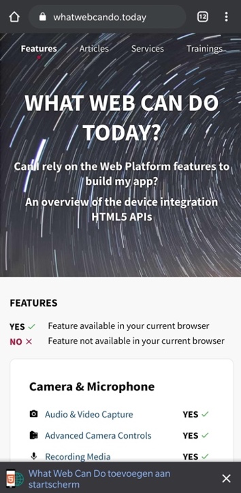
\includegraphics[width=35mm]{./img/installation_android.png}
			\caption{schermafbeelding van het installatieproces op Android 10}
			\label{A2HSExperienceIOS}
		\end{figure}
	
	
		De integratie van de ingebouwde slimme assistent is op iOS beperkter dan op Android. Als een applicatie geïnstalleerd is op een Android-toestel, kan Google assistant deze openen aan de hand van een stemcommando. Siri heeft deze functionaliteit niet.
		\autocite{Lathiya2020}
		
		\newpage
		\subparagraph{conclusie}
		
			Er kan geconcludeerd worden dat Android meer open staat voor intergraties met PWA's dan iOS. In deze trend lijkt er niet direct verandering te komen. Google, de ontwikkelaar van Android, is vaak de eerste om nieuwe web API's te ondersteunen.
			
			Langs de andere kant is iOS vaak het laatste besturingssyteem die ondersteuning zal aanbieden voor een web API.
	
	
	\subsubsection{Desktop besturingssystemen}
		Bij deze vergelijking zullen enkel Windows en macOS in beschouwing genomen worden. Andere besturingssysteem hebben relatief gezien niet veel gebruikers. 88,14\% van de computers werkt op Windows en 9,42\% werkt op macOS. Slechts 2,44\% van de computers maakt gebruik van andere besturingssystemen.
		\autocite{netMarketShare2020}
		
		Microsoft wil PWA's zo goed mogelijk ondersteunen. Ze zijn zelf ook PWA's aan het ontwikkelen. Een voorbeeld hiervan is Outlook, de populaire online e-mail-client kan nu ook geïnstalleerd worden als PWA.
		\autocite{Microsoft2020a}
		
		PWA's kunnen ook zonder aanpassingen in de Windows store geplaatst worden. Deze applicatie kan dan door alle Windows-toestellen gedownload worden. Er zijn verschillende toestellen die gebruik maken van deze store:
		\begin{itemize}
			\item	Windows 10 toestellen
			\item	Windows S toestellen
			\item	Xbox
			\item	Microsoft Hololens 
		\end{itemize}
		
		Windows gaat nog een stap verder dan dit. Het gaat zelf op zoek naar PWA's op het internet en zal deze automatisch toevoegen aan de Windows store. Dit kan wel tegengegaan worden als de uitgever van de PWA dit niet wil.
		\autocite{Gustafson2017} \autocite{Gustafson2017a}
		
		Als een PWA geïnstalleerd wordt op Windows zal deze zich gedragen als een volwaardig programma. De PWA zal opgestart worden in zijn eigen venster. Figuur \ref{fig:screenSearchWin} toont dat de applicatie ook gevonden kan worden met een zoekopdracht vanuit het startmenu. De applicatie kan ook toegevoegd worden aan de taakbalk en aan het bureaublad.
		
		\newpage
		\begin{figure}[H]
			\centering
			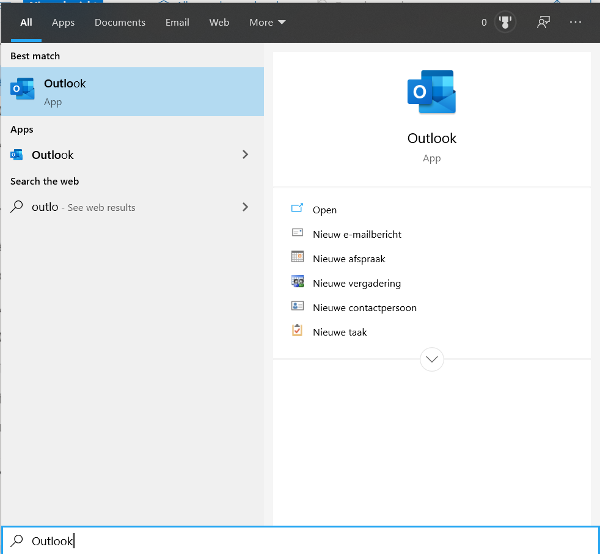
\includegraphics[width=75mm]{./img/Outlook_search_windows.png}
			\caption{schermafbeelding van de zoekresultaten van “Outlook” op Windows 10}
			\label{fig:screenSearchWin}
		\end{figure}
		
		
		De tool PWABuilder die gebruikt kan worden om een PWA in de populaire mobiele app-stores te krijgen, is ook ontwikkeld door Microsoft.
		\autocite{PWAbuilder2020}
		
		Microsoft heeft ook een uitgebreide documentatie die ontwikkelaars helpen bij het ontwikkelen van PWA's.
		\autocite{Microsoft2020b}
		
		
		Apple biedt weinig ondersteuning voor PWA's in zijn mobiele besturingssystemen. Deze trend zet zich door op de besturingssystemen voor desktops. In de standaardbrowser, Safari, van de toestellen kan een PWA niet geïnstalleerd worden. Als de gebruiker Google Chrome gebruikt, kan een PWA wel geïnstalleerd worden. Als deze geïnstalleerd is, kan de applicatie ook gevonden worden in een “spotlight search”. Dit is te zien in figuur \ref{fig:screenSearchmac}? De applicatie kan ook vastgemaakt worden aan het dock.
		
		\begin{figure}[H]
			\centering
			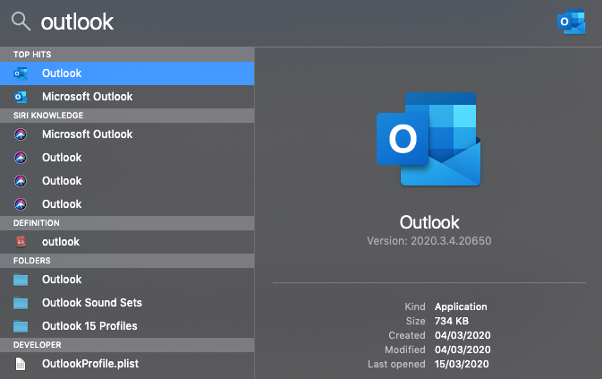
\includegraphics[width=75mm]{./img/Outlook_search_mac.png}
			\caption{schermafbeelding van de zoekresultaten van “Outlook” op macOS}
			\label{fig:screenSearchmac}
		\end{figure}
		
		De algemene trend waarbij Apple PWA's bewust niet ondersteunt, lijkt niet snel te veranderen. John Wilander, een ontwikkelaar binnen Apple, bekritiseerde openlijk PWA's als een technologie die van Google is en dat dit niet in de planning zit van Apple. 
		\autocite{Wilander2019}
		
		
		\subparagraph{Conclusie}
		Er kan geconcludeerd worden dat Windows en macOS een volledig andere filosofie hebben als het aankomt op PWA's. 
		
		Windows probeert een zo goed mogelijke ondersteuning te geven aan PWA's. PWA's worden binnen Windows behandeld als een volwaardig programma. Als een PWA geïnstalleerd is, is het moeilijk te onderscheiden van een ander native programma.
		PWA's zijn binnen Windows ook eenvoudig om te installeren.
		Micorosoft probeert ontwikkelaars ook te ondersteunen in het ontwikkelen van PWA's. Dit doen ze door een uitgebreide documentatie en tools aan te bieden.
		
		Apple daarentegen is meer gesloten voor PWA's. Vanuit de standaard browser kunnen er helemaal geen PWA's geïnstalleerd worden. Via Google Chrome is dit wel mogelijk.
		
\section{Waarom een PWA}

In dit onderdeel van de literatuurstudie zal er onderzocht worden wat de redenen zijn om wel een PWA te ontwikkelen voor een project. De voordelen zullen bekeken worden in vergelijking met traditionele webapplicaties en native applicaties.
\autocite{TandelSunil2018}


\subsection{Bereik}
	Volgens Google heeft Google Chrome meer dan 1 miljard mobiele gebruikers. In 2016 was dit nog maar 400 miljoen. Steeds meer mensen gebruiken hun smartphone om op zoek te gaan naar informatie. 
	
	\autocite{Nath2017}
	
	Data toont aan dat gebruikers nog steeds 87\% van hun tijd op hun smartphone spenderen in native applicaties, van deze 87\% wordt 80\% van de tijd in slechts 3 verschillende applicaties gespendeerd. Terwijl er veel tijd besteed wordt in native applicaties, is het toch heel moeilijk om tijd te krijgen van de gebruiker om jouw applicatie te gebruiken.
	
	De acquisitie is bij het web ook groter dan bij native applicaties. De gemiddelde gebruiker download 0 nieuwe applicaties per maand. 
	
	Op het web, waar slechts 13\% van de tijd van de mobiele gebruikers besteed wordt, worden er echter maandelijks ongeveer 100 websites bezocht. Hier is er voor bedrijven dus een kans om een gebruiker jouw platform te laten ontdekken en nieuwe gebruikers te winnen.
	
	\autocite{GoogleChromeDevelopers2017}
	

\subsection{Platformonafhankelijkheid }
	Een van de grootste voordelen van het web is dat het platformonafhankelijk is. Een webapplicatie hoeft maar eenmaal ontwikkeld te worden en kan dan op meerdere platformen gebruikt worden. Het web is ook niet gebonden aan deze conventionele platformen. De dag van vandaag zijn meer en meer toestellen zoals televisies, game-consoles en e-readers verbonden met het internet. 
	
	PWA’s kunnen meer geavanceerde functionaliteiten implementeren dan een traditionele webapplicatie. Bepaalde functionaliteiten zijn wel platformafhankelijk. Een functionaliteit die kan toegevoegd worden is push-notifications. Zoals aangetoond in vorig hoofdstuk zal dit niet werken op IOS-toestellen. De PWA zal wel nog werken op IOS maar zal niet genieten van deze functionaliteit. PWA’s zijn dus gedeeltelijk platformonafhankelijk.
	
	Bij native ontwikkeling zijn er vaak verschillende codebases voor elk platform die het ondersteunt. Er zijn technologieën die dit proberen op te lossen zoals React Native. Maar ook hier moet er voor bepaalde delen nog native code geschreven worden per platform. Native applicaties zijn dus niet platformonafhankelijk. 


\subsection{Omzet}
	Conversion rate is een meeteenheid die gebruikt wordt om de omzet van een website te peilen. Hoe hoger de conversion rate hoe beter. De conversion rate wordt bepaald door het aantal ‘conversions’ die een website heeft ten opzichte van het aantal bezoekers. Een conversion kan voor elke website anders gedefinieerd worden. Voor een e-commerce website zal dit vaak een aankoop zijn. Voor andere websites kan dit het aanmelden van de gebruiker op de nieuwsbrief zijn.
	\autocite{GoogleSupport2020}
	
	Nikkei is een nieuws-website die in 2018 zijn website ombouwde tot een PWA.  Door het gebruikmaken van serviceworkers konden ze de laadtijd van hun website drastisch verlagen (14 seconden sneller – van +- 20 seconden naar +-6 seconden). Dit had als gevolg dat gebruikers steeds vaker naar Nikkei gingen als nieuwsbron. 
	
	De conversion rate steeg met 58\% (premium abonnement) en er was een stijging van 49\% in het aantal dagelijkse gebruikers. Deze gebruikers lazen gemiddeld het dubbel aantal artikelen dan voordien. 
	\autocite{Developers2018}
	
	Dit voorbeeld toont aan dat de omzet met een PWA hoger kan zijn dan bij traditionele webapplicaties.
	
	Met native applicaties kan er nog steeds een meer gepersonaliseerde ervaring geboden worden en zal er gemiddeld gezien ook een hogere conversion rate zijn. Maar PWA’s scoren beter dan traditionele websites.
	\autocite{Anastasia2019}
	

\subsection{Bundle size}

	bundle size is de grootte van de applicatie als deze geïnstalleerd wordt. Het is positief om een zo klein mogelijke zoals televisies, game consoles en e-readers.  bundle size te hebben.
	\autocite{Scott2019}
	
	Tinder besliste om zijn service ook aan te bieden als een PWA. Tinder slaagde erin om alle functionaliteiten die hun native applicaties hebben over te nemen in de PWA. Ze slaagden hierin door gebruik te maken van verschillende web API’s. 
	\autocite{Osmani2017}
	
	Een van de grootste voordelen is dat de PWA (versie 118) op het moment van schrijven slechts een grootte heeft van 397kb. De native Androidapplicatie (versie 11.8.1) daarentegen neemt 130mb in beslag op een toestel.
	
	In Westerse landen is dit handig, maar zal het zelden bepalen of een gebruiker een applicatie effectief gebruikt. In andere markten zoals Afrika is dit heel belangrijk. De toestellen die er gebruikt worden zijn vaak verouderd en hebben mindere specificaties dan dat de toestellen gebruikt in het Westen. 
	
	De gemiddelde prijs van de top 5 meest verkochte smartphones in Afrika was 135,6 USD. Deze toestellen beschikken vaak over slechts 8 of 16GB opslagruimte. 
	\autocite{netAdmin2017}
	
	Slechts 7\% van Afrika beschikt over een 4g connectie. De andere gebieden moeten het vaak doen met een tragere 3g connectie.	
	
	% https://www.gsmaintelligence.com/research/?file=36b5ca079193fa82332d09063d3595b5&download – 28 februari
	
	
	%TODO: bron toevoegen  - zie word doc - server was down
	
	************	BRON TOEVOEGEN  - ZIE WORD DOCUMENT - SERVER WAS DOWN **************
	
	Hier is het dus zeer handig en belangrijk om zo klein mogelijke applicaties te leveren.
	
	\begin{figure}[H]
		\centering
		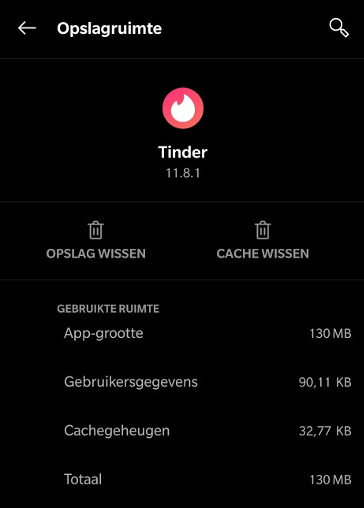
\includegraphics{./img/tinder_native.png}
		\caption{Android native applicatie versie 11.8.1}
	\end{figure}
	
	\begin{figure}[H]
		\centering
		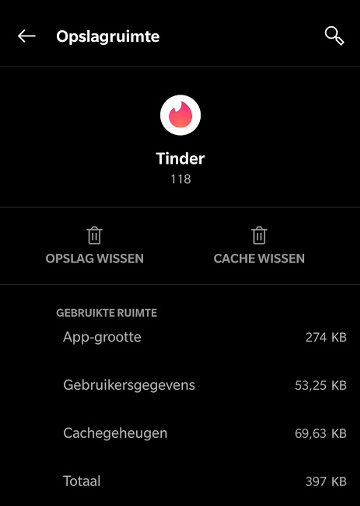
\includegraphics{./img/tinder_pwa.png}
		\caption{PWA-versie 118}
	\end{figure}





\subsection{Offline gebruik}
	Een webapplicatie kan nu geïmplementeerd worden met een ‘offline-first’ benadering. Offline first is gelijkaardig aan progressive enhancement. Eerst wordt er een applicatie gebouwd die volledig offline beschikbaar is, die vervolgens uitgebreid met online functionaliteiten. 
	
	Door gebruik te maken van de fetch API in een service worker kunnen API-calls onderschept worden. De service worker kan vervolgens controleren als de gebruiker online is. Als dit niet het geval is, kan de service worker de API-call annuleren en zelf een antwoord sturen met een 200-status en een melding dat er geen internet is. Op basis hiervan kan er een gepaste boodschap getoond worden aan de gebruiker en zal de applicatie niet crashen.
	\autocite{Developers2019a}
	
	Data van API-calls kan ook lokaal opgeslagen worden. Als een bepaalde API-call herhaald wordt, kan in plaats van de backend aan te spreken de lokale data gebruikt worden. Dit zal de ervaring voor gebruikers met een zwakke of inconsistente netwerk-connectie verbeteren.
	\autocite{Vanhala2017}
	
	
\subsection{Betrokkenheid}
	Een van de redenen om een native applicatie te maken, was vaak betrokkenheid. Via het web heb je een groot bereik, maar gebruikers op een bepaald platform houden was moeilijk met de
	
	\autocite{Google2019}


	
	Push notifications zijn meldingen die op het toestel van een gebruiker tevoorschijn komen. Deze worden verstuurd van een server en zijn dus niet afhankelijk van input van een gebruiker. Door gebruik te maken van de Push API en de Notifications API kunnen deze meldingen gebruikt worden bij een PWA.
	
	Push notifications kunnen gebruikers herinneren om een bepaalde applicatie terug te gebruiken. 
	
	Push notifications kunnen ook gebruikt worden om de conversion rate te verhogen. Bijvoorbeeld bij een e-commerce platform kan er een melding gestuurd worden als de klant items in zijn mandje heeft geplaatst maar deze nog niet heeft besteld.
	
	\autocite{Gaunt2020}
	\autocite{Hiltunen2018}

	
	Als een webapplicatie voldoet aan de criteria (zie hoofdstuk “wat is een PWA”) van een PWA, kan deze toegevoegd worden aan het startscherm van een toestel. Hierdoor wordt het voor de gebruiker gemakkelijker om een PWA herhaaldelijk te gebruiken. Als een applicatie wordt geopend vanaf het startscherm, kan deze het volledige scherm gebruiken en zullen adresbalk en andere tools van de browser weggelaten worden. Dit zorgt ervoor dat de PWA meer zal aanvoelen als een native applicatie dan een website.
	
	Door deze nieuwe functionaliteiten toe te voegen, is de betrokkenheid van een PWA groter dan die van een traditionele webapplicatie. Nog niet alle functies die beschikbaar zijn voor native applicaties zijn beschikbaar voor PWA’s.
	

\subsection{Kost}
	Het ontwikkelen van native applicaties is niet goedkoop. Services zoals Spotify moeten native applicaties ontwikkelen voor verschillende platformen (MAC OS, Windows, IOS, Android, Linux, ChromeOS).
	
	Het creëren van een digitaal product voor verschillende platformen is vaak te duur voor een kleiner of startend bedrijf. Progressive web apps kunnen hier een oplossing bieden. Een PWA kan geïnstalleerd worden op al de bovenstaande platformen. In plaats van eenzelfde applicatie te bouwen voor verschillende platformen, kan er met PWA’s dus 1 applicatie geschreven worden die op verschillende platformen kan gebruikt worden.
	
	Spotify implementeerde zijn service ook als een PWA. \autocite{Spotify2020} Al de functies die op de native applicaties beschikbaar zijn, zijn ook beschikbaar via deze webapplicatie. Enkel de offlinefunctie is (nog) niet geïmplementeerd. Ook het gebruik van de functietoetsen op het toetsenbord van een desktop is niet ondersteund.
	
	\autocite{Vu2019}
	
	
\subsection{Deployment}

	Het uitgeven van een PWA is ook een stuk gemakkelijker en goedkoper dan het verdelen van native applicaties door middel van de verschillende app-stores. 
	Om een applicatie te publiceren in de Apple app-store moet de ontwikkelaar een “Apple developer” account hebben. Dit kost 99 euro per jaar. 
	\autocite{Apple2020b}
	
	Ook het publiceren van een applicatie op de Google play store is niet gratis. De uitgever moet een developer account hebben bij Google play. Dit kost eenmalig 25 USD.
	Elke app-store (Windows, Apple, Android, Chrome, …) heeft zijn eigen specifieke eisen en kosten om een applicatie te kunnen uploaden. Bij een PWA hoeft er slechts één applicatie online gezet te worden. Deze moet niet gevalideerd worden door andere partijen. 
	\autocite{GooglePlay2020}
	
	Het publiceren van een applicatie op de Windows store is gratis.
	
	Het publiceren van een PWA is meestal ook niet gratis. Het online brengen van een website heeft meestal 2 kosten: enerzijds aankoop van een domein en anderzijds de hosting van een applicatie met https-verbinding. Deze kosten zijn ook nodig bij traditionele webapplicaties.
	Een domein aankopen via de website versio.nl kost 28,95 euro voor vijf jaar.
	\autocite{Versio2020}
	
	Het hosten van een statische applicatie kan via bepaalde platformen kosteloos gebeuren. Voorbeelden van deze platformen zijn Firebase \autocite{Firebase2020} en Netlify \autocite{Netflify2020}. 	
	Deze platformen bieden ook gratis SSL-certificaten aan zodat er een HTTPS-connectie is. 
	
	De kost om een PWA online te brengen is dus even hoog als bij traditionele websites. De kost is wel lager dan bij native applicaties. 	
	
	De kost is niet het enige voordeel van het online brengen van PWA’s ten opzichte van native applicaties. Als een applicatie gepubliceerd wordt in de Apple App store of in de Google Play Store dan moeten deze voldoen aan een groot aantal richtlijnen. Bij het uploaden van een applicatie wordt deze eerst gecontroleerd door Apple en Google of deze wel voldoet aan deze richtlijnen. 
	\autocite{Apple2020c}
	\autocite{GooglePlay2020a}
	
	Dit betekent dus dat niet elke applicatie gepubliceerd kan worden in deze app-stores. Een PWA moet niet gevalideerd worden door een overkoepelend bedrijf. Elke applicatie die de ontwikkelaar maakt kan dus gepubliceerd worden.
	Een ander gevolg is dat het gemiddeld 72 uur duurt om een app te laten valideren door beide app-stores. Dit is slechts een gemiddelde, want dit kan uitlopen tot een week en langer.
	\autocite{Siddiqui2019}
	
	Dit is een vertraging die webapplicaties en PWA’s niet hebben.
	
\subsection{Updates}

	Als een PWA bezocht wordt, zal deze steeds de meeste recente versie tonen. Als er een update moet gebeuren, kan de ontwikkelaar kiezen om dit wel of niet aan de gebruiker te laten weten. 	
	\autocite{Hume2018}
	
	Kleinere updates die de gebruiker niet zal opmerken, kunnen uitgevoerd worden zonder dat de gebruiker dit weet.
	 \autocite{Sanderson2020}
	 
	Als er grotere updates zijn, is het een betere user experience om de gebruiker te informeren dat er een update zal uitgevoerd worden.
	\autocite{Wicki2017}
	 
	De ontwikkelaar heeft dus volledige vrijheid in hoe hij omgaat met updates. De gebruiker kan steeds genieten van de laatste versie van de applicatie zonder dat hij deze zelf manueel moet updaten. Deze ervaring is dezelfde voor traditionele websites.
	
	Zowel Android als IOS hebben een functionaliteit om hun applicaties automatisch te updaten. Deze functionaliteit werkt echter enkel voor kleine incrementele updates. Als de applicatie functionaliteiten aanpast, toevoegt of verwijdert, moet deze app nog steeds manueel geüpdatet worden via de app-store. Als ontwikkelaar heb je dus geen controle over welke versie de gebruiker aan het gebruiken is.
	
	\autocite{Apple2020d}
	\autocite{AndroidDevelopers2020}
		

\subsection{Conclusie}
	\begin{table}[H]
		\centering
		\begin{tabular}{llll}
			                         			  & Web applicatie 	 				 & PWA								 & Native applicatie \\
			Bereik                   		   & \cellcolor{green!40}      		 & \cellcolor{green!40}			& \cellcolor{red!50}\\
			Platformonafhankelijkheid   & \cellcolor{green!40}      	  & \cellcolor{orange!50}		& \cellcolor{red!50}\\
			Omzet   						  & \cellcolor{red!50}      		 & \cellcolor{orange!50}		& \cellcolor{green!40}\\
			Bundle size						  & niet van toepassing      		& \cellcolor{green!40}		   & \cellcolor{red!50}\\
			Offline gebruik					 & \cellcolor{red!50}      		    & \cellcolor{green!40}			& \cellcolor{green!40}\\
			Betrokkenheid 					& \cellcolor{red!50}      		   & \cellcolor{orange!50}		 & \cellcolor{green!40}\\
			Kost 								& niet van toepassing     		  & \cellcolor{green!40}		 & \cellcolor{red!50}\\
			Deployment 						& \cellcolor{green!40}      	  & \cellcolor{green!40}		 & \cellcolor{red!50}\\
			Updates	   						& \cellcolor{green!40}      	  & \cellcolor{green!40}		 & \cellcolor{red!50}\\
		\end{tabular}
		\caption{concluderende tabel 'waarom een PWA'}
	\end{table}
	
	\begin{table}[H]
		\centering
		\begin{tabular}{lll}
			Positief \cellcolor{green!40} & Matig \cellcolor{orange!50} & Negatief  \cellcolor{red!50}
		\end{tabular}
	\end{table}
	
	

\clearpage
\section{Beperkingen van een PWA}
\label{ch: beperkingenPWA}

Zoals aangetoond in de sectie ‘besturingssystemen en '’ kan het web gebruik maken van verschillenden hardware-functies van een toestel. Onderzoek toont echter dat voor sommige toepassingen een PWA niet de oplossing is.
\autocite{Malavolta2016}


\subsection{Cameragebruik}
	Onderzoek van Rebecca Fransson toont aan dat de video’s die opgenomen worden met de mediaCapture API van een veel lagere kwaliteit zijn. Ook duurde het proces van het opnemen van een video statistisch significant langer. De methode waarbij er gebruik gemaakt wordt van de mediaCapture API is wel ondersteund door alle populaire browsers.
	
	De resultaten waarbij video’s opgenomen worden met de nieuwere ImageCaptureAPI waren een stuk beter en benaderden de kwaliteit van een native applicatie. Het probleem bij deze techniek is dat deze API enkel ondersteund wordt door Google Chrome.
	\autocite{Fransson2017}
	

\subsection{Controle over platformen}
	
	Met native applicaties kan de ontwikkelaar kiezen voor welke platformen hij de applicatie zal publiceren. Het web, en dus ook ', kunnen van op verschillende toestellen bezocht worden. Dit is een van de voordelen van het web. Dit zorgt er echter voor dat de ontwikkelaar rekening moet houden met de verschillende mogelijkheden van de toestellen. Er kan een applicatie geschreven worden die afhankelijk is van een cameratoepassing. Toestellen die geen camera hebben (oudere telefoons, smart-tv, desktops, …) kunnen perfect op deze site terecht komen. Helaas zullen zij niet kunnen genieten van de functionaliteit van de applicatie.
	
	Een webapplicatie kan geopend worden op een scherm van enkele centimeters groot. Deze zelfde applicatie kan ook geopend worden op een groot televisiescherm. De ontwikkelaar moet ervoor zorgen dat de applicatie op al deze groottes bruikbaar is.
	
	
\subsection{Functies van een besturingssysteem}

	Integratie in het besturingssysteem is ook niet mogelijk. Een PWA kan dan wel geïnstalleerd worden en toegevoegd worden aan het startscherm zodat het aanvoelt als een native app, maar bepaalde toepassingen zijn enkel mogelijk met native applicaties.
	
	Een PWA kan bijvoorbeeld geen widgets plaatsen op het startscherm van een Android toestel. 
	
	De instellingen van een toestel kunnen ook niet gemanipuleerd worden vanuit een PWA. Native applicaties kunnen bepaalde acties uitvoeren door de ingebouwde smart assistant (Google Assistant voor Android, Siri voor IOS), Deze assistenten kunnen nog niet interageren met geïnstalleerde '.
	
	Zoals aangetoond in de sectie ‘besturingssystemen en '’ kan een PWA ook geen toegang krijgen tot de alarmen van een toestel.
	
	Toegang tot de hardware van toestellen is nog steeds beperkt. Er bestaan reeds heel wat web-API’s voor het aanspreken van deze sensoren. De ondersteuning van deze technologieën is nog niet goed (zie hoofdstuk \ref{ch: Besturingssystemen en PWA's}).
	De toegang tot persoonlijke informatie is ook beperkt. Er is voor webapplicaties geen toegang tot belgeschiedenis, berichten, kalender, … Dit is data waar native applicaties wel gebruik kunnen van maken.
	\autocite{Brousek2017}
	
\subsection{Browserondersteuning}

	De ondersteuning van de functionaliteiten die een PWA aanbiedt, is niet op elke browser gelijk. Alle moderne browsers ondersteunen service workers, maar meer specifieke functionaliteiten zoals push-notificaties zijn nog niet overal beschikbaar.
	
	
\subsection{Aanwezigheid in app-stores}
	PWA zijn gemakkelijk te vinden via het web, maar bepaalde potentiële gebruikers zullen een applicatie in een app-store verwachten. Deze zal hier echter niet te vinden zijn.
	
	
\subsection{Conclusie}
	\begin{table}[H]
		\centering
		\begin{tabular}{lp{35mm}lp{35mm}lp{35mm}l}
			                         			  & Web applicatie 	 				 & PWA								 & Native applicatie \\
			Cameragebruik                  & \cellcolor{red!50}      		 & \cellcolor{red!50}			& \cellcolor{green!40}\\
			Controle over platformen   	& \cellcolor{red!50}      	  & \cellcolor{red!50}		& \cellcolor{green!40}\\
			Functies besturingssysteem  & \cellcolor{red!50}      		 & \cellcolor{orange!50}		& \cellcolor{green!40}\\
			Browserondersteuning		 & \cellcolor{green!40}     		& \cellcolor{orange!50}		   &niet van toepassing\\
			Aanwezigheid in app-stores	 & \cellcolor{red!50}      		    & \cellcolor{red!50}			& \cellcolor{green!40}\\
		
		\end{tabular}
		\caption{concluderende tabel 'beperkingen van een PWA'}
	\end{table}
	
	\begin{table}[H]
		\centering
		\begin{tabular}{lll}
			Positief \cellcolor{green!40} & Matig \cellcolor{orange!50} & Negatief  \cellcolor{red!50}
		\end{tabular}
	\end{table}
\clearpage
\section{Tools voor het ontwikkelen van een PWA}


\subsection{Lighthouse}

	Lighthouse is een tool die een audit zal uitvoeren op een website en een rapport zal uitgeven. Dit rapport kan een ontwikkelaar veel interessante informatie geven om de ervaring van deze website te verbeteren. De audit geeft inzichten op vlak van:
	
	\begin{itemize}
		\item	Prestaties
		\item	Toegankelijkheid
		\item	Best practices
		\item	SEO
		\item   PWA
	\end{itemize}
	
	\autocite{Lighthouse2020}
	
	Voor elk van deze onderdelen, op 'PWA' na, zal er een score op 100 gegenereerd worden. De audit zal ook voorstellen doen om deze scores te verhogen en de ervaring voor de eindgebruiker dus te verbeteren.
	
	Voor het onderdeel PWA zal er een checklist gegenereerd worden met items waaraan de applicatie moet voldoen om geïnstalleerd te kunnen worden op een toestel. Dit onderdeel wordt opgedeeld in drie delen: 'fast and reliable', 'installable' en 'PWA optimized'.
	
	
	\subsubsection{Fast and reliable}
		De eerste metriek die getest wordt, is de iOS van de website. Er wordt zowel gekeken naar de iOS waarmee de eerste inhoud op de pagina komt (FMP - first meaningful paint) maar ook naar wanneer de gebruiker voor het eerst kan interageren met de website (TTI - time to interactive).
		\autocite{web.dev2020}
		
		Vervolgens worden de offline capaciteiten van de website getest. Er wordt getest of de huidige pagina en startpagina reageren met een antwoord die de statuscode 200 bevat als er geen internetverbinding is. Dit wil zeggen dat er een succesvol antwoord was en dat de website dus offline kan werken.
	
	
	\subsubsection{Installable}
	
		In dit deel van de PWA-audit zal gecontroleerd worden of de website voldoet aan alle vereisten om geïnstalleerd te kunnen worden. Dit zijn:
		\begin{itemize}
			\item	Er moet een HTTPS-verbinding zijn.
			\item	Er moet een service worker geregistreerd worden.
			\item	Er moet een minimum app-manifest zijn.
		\end{itemize}
		\autocite{web.dev2020a}
		
	
	\subsubsection{PWA optimized}
	
		In dit onderdeel wordt er gecontroleerd op kleine optimalisaties die een betere gebruikers-ervaring kunnen bieden. 
		Een voorbeeld hiervan is dat als een gebruiker naar de HTTP-versie van een website surft, hij herleid wordt naar HTTPS-versie.
		
		Een andere controle is dat het themakleur van de applicatie is ingesteld. Dit kan gebeuren in de app-manifest. Ook dit zorgt voor een betere user experience en een meer native feeling. Deze app manifest moet een specifiek icoon bevatten voor de iPhone. Ook deze controle wordt uitgevoerd.
		
		
		\begin{figure}[H]
			\centering
			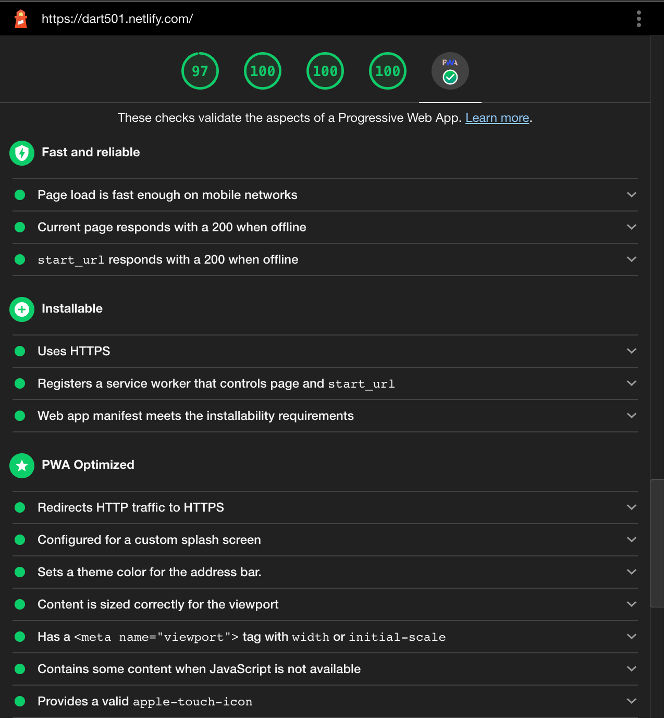
\includegraphics{./img/lighthouse.png}
			\caption{screenshot van het onderdeel 'PWA' in een lighthouse audit op de site \href{ https://dart501.netlify.com}{dart501.netlify.com} }
		\end{figure}
		
		

\subsection{Workbox}

	Workbox is een verzameling van libraries die helpt bij het ontwikkelen van service worker gerelateerde functionaliteiten.
	
	Workbox wil het gemakkelijker maken voor de ontwikkelaars om middelen te cachen en op deze manier een snellere en minder netwerk-afhankelijke applicatie te maken.
	
	Het debuggen van een PWA kan ook moeilijk worden omdat code lokaal opgeslagen kan worden en je als ontwikkelaar niet altijd weet welke versie van de code voor een bepaald gedrag zorgt. Ook om deze problemen te debuggen voorziet Workbox tools.
	\autocite{Workbox2020}
	

\subsection{PWAbuilder}

	Pwabuilder.com is een website, gecreëerd werd door Microsoft, die ervoor zorgt dat een PWA toch in de app-stores kan terechtkomen. Als ontwikkelaar moet je juist een link van een PWA opgeven en de tool maakt van deze PWA vier pakketten die kunnen geüpload worden naar hun bijhorende app-store. 
	
	Volgende platformen zijn ondersteund:
	
	\begin{itemize}
		\item	Android
		\item	Samsung (eigen Samsung store)
		\item	Windows
		\item	iOS
	\end{itemize}
	\autocite{PWAbuilder2020}
	
	
\subsection{Chrome developer tools}
	De Chrome developer tools bieden een grote hulp bij het ontwikkelen van webapplicaties.
	
	Chrome zorgt ervoor dat er eenvoudig gecachete items tijdelijk verwijderd kunnen worden. Hierdoor kan de ontwikkelaar testen of een service worker de juiste bestanden offline beschikbaar maakt.
	
	Google Chrome biedt tools om eenvoudig een website offline te testen of om bepaalde service workers uit te schakelen.
	Ook de volledigheid van het app-manifest bestand kan in de Chrome developer tools bekeken worden.
	
	De Chrome developer tools hebben ook een sectie waar de status van de service worker kan bekeken en gemanipuleerd worden.
	\autocite{Developers2019b}
	

	
	




